\documentclass[12pt]{article}

\usepackage[utf8]{inputenc}
\usepackage{CJKutf8}
\usepackage{algorithm}
\usepackage{algorithmicx}
\usepackage{amsmath}
\usepackage{algpseudocode}
\usepackage{amssymb}
\usepackage{pdfpages}

\newcommand{\remark}[1]{\textcolor{red}{#1}}
%\newcommand{\parencite}[1]{\cite{#1}}

%\usepackage{natbib}
\usepackage{graphicx}
\usepackage{geometry}
\usepackage{setspace}

\geometry{a4paper,scale=0.75}

\renewcommand{\figurename}{图}
\renewcommand{\contentsname}{目录}


\title{大规模可视化数据管理 \\ 前沿综述报告}
\author{主\ \ 编\ \ \ 袁晓如 \\ 编\ \ 者\ \ (按拼音顺序)\ \ \ 李彦达\ \ \ 刘\ \ 灿\ \ \ 杨昌和\ \ \ 张\ \ 江}
\date{2020\ 年\ 1\ 月\ \ \ 第\ 1\ 版}

\usepackage[backend = biber]{biblatex} 
\addbibresource{references.bib}

\begin{document}
\begin{spacing}{1.5}
\begin{CJK*}{UTF8}{gbsn}
%\maketitle
\renewcommand{\refname}{参考文献}

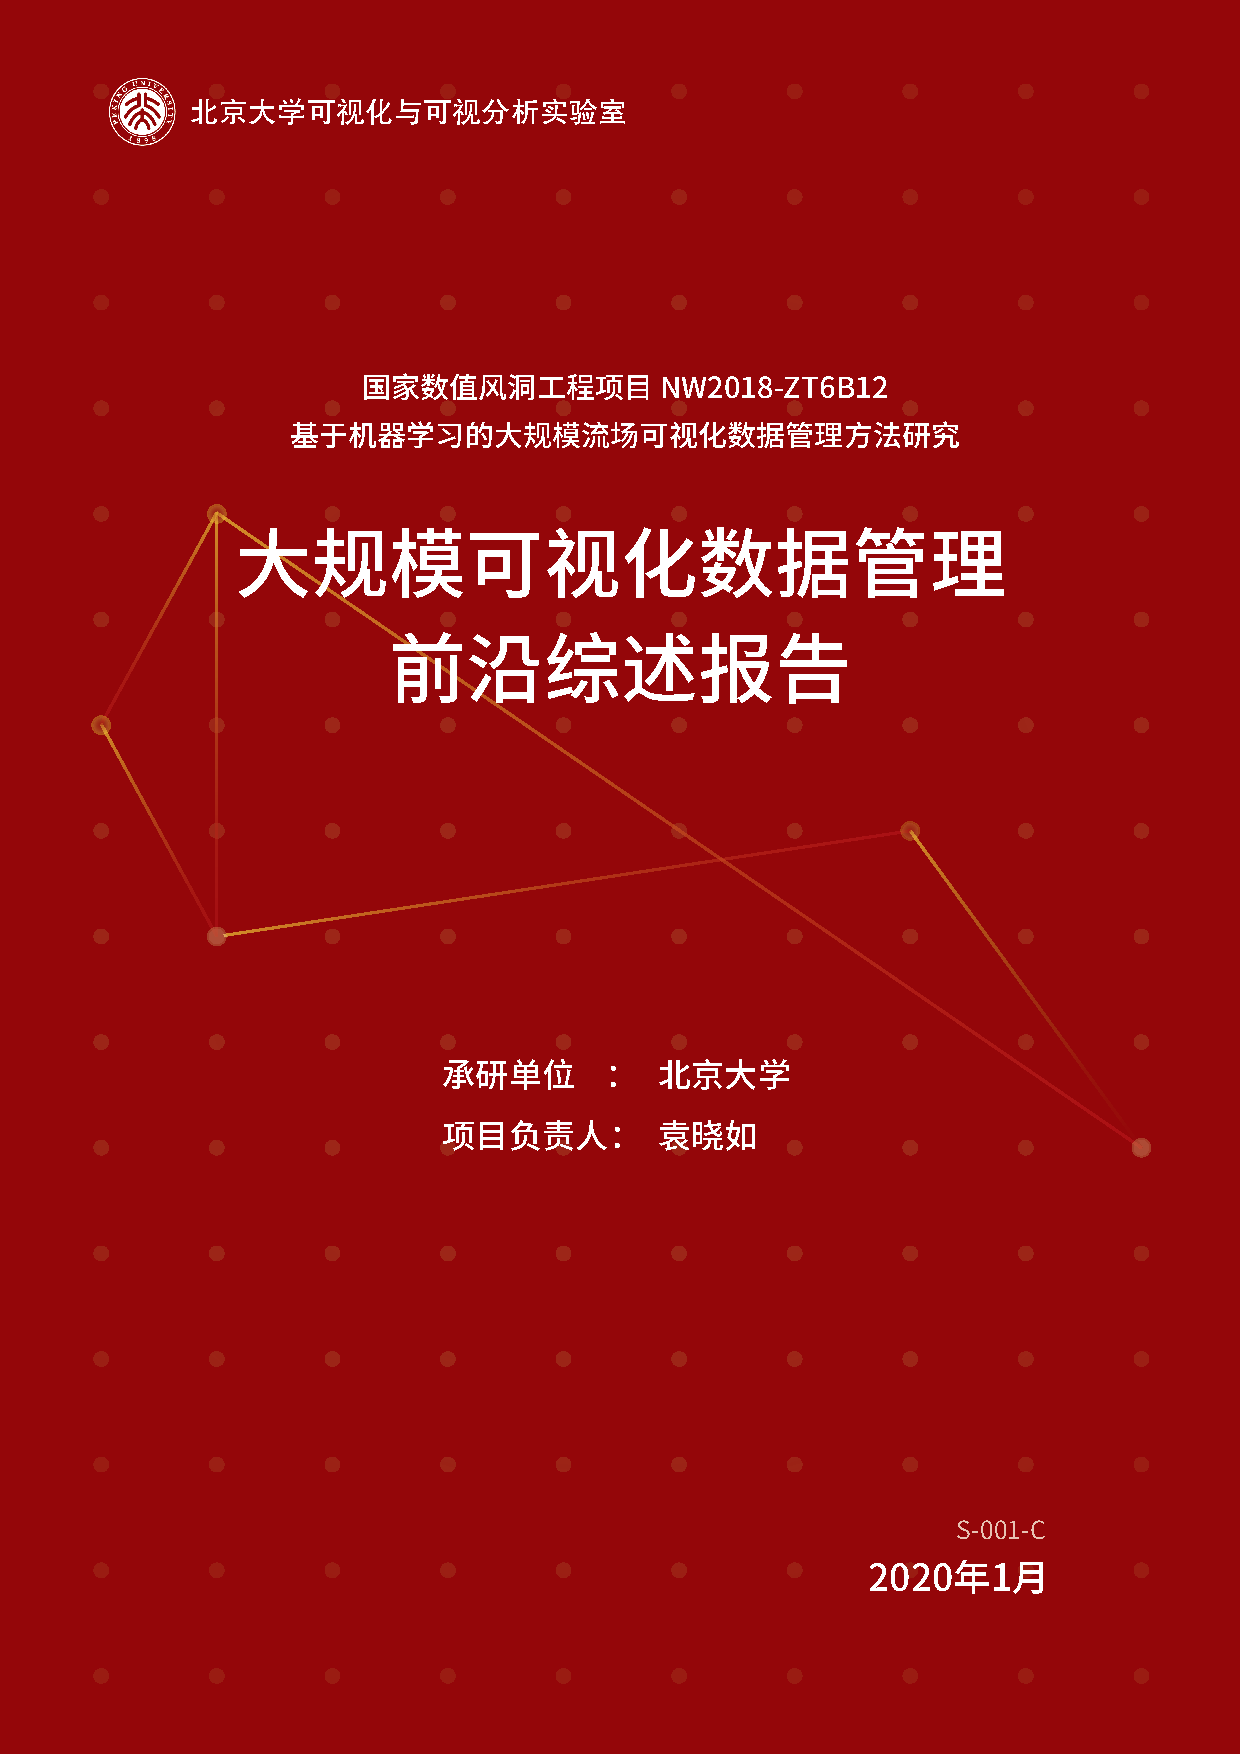
\includepdf[pages={1}]{image/firstCover/firstCover.pdf}

\clearpage
\maketitle

\clearpage
\tableofcontents

\clearpage
\section{背景}
随着科学、工程、生物医学等领域的不断发展,研究者们往往需要面对大量来自燃烧、气候、航空等模型的模拟和观测数据,并需要从中发现有意义的规律,以帮助人们更好地理解现实世界中的复杂现象及其动态演变过程。

人类通过模拟、观测到大量的科学数据。科学数据包括标量场数据和矢量场数据。这些数据往往是通过医学扫描(如核磁、CT等)、计算流体动力学等数值模拟获得。并且通常具有时变(time-varying)、多变量(multivariate)等特性。科学家们需要对这些数据进行有效的可视化并分析出其中存在的特征,从而解释现象或者验证假设。

然而,科学家通过数值模拟等方式得到的数据规模越来越大。其内部结构也越来越复杂。传统的可视化方法遇到了越来越多的挑战。比如,仅仅是加载数据进入处理器也非易事,更遑论对数据进行各种操作。这需要更高效的数据组织方法来支持大规模科学数据的可视化。

科学数据管理通常面临着以下挑战,可以归纳为3个V。

\begin{itemize}

\item \textbf{Volume(数据规模增大)}

巨大的规模让科学数据难以存储、管理、传递、分析和可视化。
传统的可视化的软件方法在大规模的数据环境下其运行时间未必能和数据规模等比增长。
这是实际的存储空间的存储是多层级地分配在不同的硬件上,其效率会随着硬件的实际限制而渐渐脱离理想状态。
尽管现代大型计算机的内存、硬盘大小有了非常快速的增长。其内存存取速度、硬盘带宽的增长速率没有赶上计算能力的增长速率。这让数据合理的组织划分变得尤为重要。

\item \textbf{Velocity(数据处理速度需求增高)}

在数据量增大的同时,人类对快速产生结果也的需求却并且随着数据量的增加而同步增加。为了能够在人类能够接受的时间内产生结果,需要有对数据更高效的处理方式,能够利用多种先进的技术。

\item \textbf{Variety(数据、任务多样性增大)}

需要处理的科学数据范畴越来越广。涉及的数据从标量,矢量,到张量。涉及的任务包括绘制体数据、迹线、特征面等,这使得难以构建通用的分析框架。对数据管理具有更为灵活的要求。

\end{itemize}

为了解决这些大规模数据量导致的问题,需要有一些对数据高效的组织方法。因此从以下几种数据处理的方式分别展开分析。
数据的I/O往往需要很大的时间负担,数据预取提前将可能被访问的数据块加载到内存中,这是解决该问题的有效手段。在科学可视化中,数据的访问根据不同任务有不同的特征,其中流场可视化由于根据流场走势需要较为复杂的模式,我们基于流场可视化对大规模科学数据中的数据预取展开分析并介绍。

除了通过数据预取,采用并行手段也是重要方式。在多线程的任务中,尽可能地让线程之间保持运算负载的均衡可以让整体运算更假高效。结合大规模科学数据可视化的特点,为了充分利用计算资源,从数据存储组织和访问方式以及在应用程序执行过程中对数据的划分和调度管理等方面进行考虑。

此外,从数据本身而言,通过数据约减技术改变数据表达形式,并降低其规模也是一种有效的处理方式。





\clearpage
\section{科学可视化典型数据流程中数据管理策略的应用}

科学可视化是科学研究中的一个跨学科研究分支。其主要关注三维现象(如建筑学、气象学、医学、生物学等)的可视化和分析探索,强调对于体、表面、场景等的逼真渲染,涵盖高维数据和时变的分析等复杂元素。科学可视化技术的目的是图形化地展示和说明科学数据,使科学家可以理解他们的数据,并从其中获得有效的启发和见解。科学可视化处理的数据对象为科学数据,通常包含具有自然几何、空间结构的数据,如洋流流场、CT扫描数据等。由于数据来源的多样性、数据采集对象本身的多变性、以及数据采集、记录的设备能力的大幅提高,科学数据通常十分复杂,隐含着十分庞大的信息,具有深刻的研究价值。同时科学可视化处理的数据完全符合当下大数据环境下被归纳中3个V的挑战,这也为分析和研究工作带来了巨大障碍,需要优良的计算策略和丰富的计算资源作为进行分析的支持。为了高效地分析和探索大规模的科学数据,科学可视化中通常需要采用多样的数据管理策略,来帮助用户有效实现的科学可视化应用,以应对不同场景下多变的研究任务。

针对这一类大规模数据的复杂任务,并行计算的模式成为了一种十分行之有效的解决方案。研究者可以更多地利用超级计算机或者并行计算集群等强大的计算资源来进行并行计算,十分有效地提升了科学可视化计算结果产出的效率。基于上述研究的解决方案,科学可视化中典型的数据流程如图\ref{fig:scivisWorkflow:pipeline}所示。整个流程的分解可以归纳为数据重组织和优化的并行计算处理两部分。原始科学数据经过数据划分和组织后基于一定策略被分配到各个进程,再经过优化的并行计算后可以生成最终的可视化结果。

\begin{figure}[h]
  \centering
  \includegraphics[width=\linewidth]{image/scivisWorkflow/pipeline.eps}
  \caption{
    科学可视化数据中处理与计算流程。
  }
  \label{fig:scivisWorkflow:pipeline}
\end{figure}

% 数据重组织
\subsection{数据重组织流程中的数据管理策略}
原始的科学数据通常完全依据其原有的语义结构进行组织,通常含有十分显著的三维的空间语义。如体数据是常见的一种数据形式,它记录了三维空间中离散网格上点的属性。构成体数据的基本单位为体素,类比于二维空间中像素的概念,一个体素表示了体数据中的三维空间中某特定部分的值。体素的值可以为标量,例如CT扫描数据、核磁共振数据等。体素的值也可以为矢量,例如流场数据等。由于大规模科学数据本身具有的复杂性,难以整块直接载入内存直接进行计算,通常需要进行数据组织上的更变,以适应并行计算环境和体系下的计算行为模式。例如在数据重组织流程中,对于原始数据的分块策略就是一种十分简单而有效的方式。这一技术通过将原始数据按照一定的策略划分为多个子数据块,或将整体的任务划分为多个任务子集,并在后续的并行计算过程中分配给不同的进程进行处理。这样的数据重组织方式有效的适应了并行计算的特性,最大化了这一计算框架下资源的利用率,因而有助于提升整个科学可视化流程的有效性。

数据约减是科学可视化数据重组织流程中一种更加精巧而有效的处理手段和技巧。不同于分块组织策略的简单的形式分离的方式,数据约减将数据从结构层面上做出完全的更替和优化,因而使得数据在后续的并行计算和处理流程中能够表现出新的特性。良好的数据约减方式需要完全的适应计算任务的需求,并针对性的提供方便的结构以支持高并行化的算法。数据约减策略对于科学可视化数据流程的的优化不仅在于其对于并行计算过程中可选的数据访问量的减少的性能提升,而是其进一步地给出的数据的高效浓缩的、抽象化的表达对于单次访问的效率的提升,这为大规模科学数据的数据查询和可视化提供了无比高效的便利。

近年来受到广泛关注的一种针对模拟计算产生的超大规模数据的可视化模式被称为原位可视化。普通的可视化计算模式将超大量级模拟产生的全部数据传递到存储设备,再经处理后用于可视化。在这个过程中,数据传输是整个系统的瓶颈,I/O将占据绝大部分的计算时间。而在原位可视化模式中,数据直接在计算后原位被缩减与前处理,再用于随后的可视化与分析。经过缩减后的数据,通常比原始数据小多个数量级,能够极大地降低数据传递和存储的开支。

使用数据约减不仅可以大大提高科学可视化的数据访问效率,还可以反过来对流场数据的访问的规律与模式进行特征抽取,来指导设计特定的数据管理与访问方法,来提高大规模科学可视化数据分析的效率与可扩展性。数据约减的管理策略可以将粗粒度的数据划分转化为细粒度划分,提高并行计算算法中任务调度和通信的粒度,提高算法的性能和可扩展性。

总的来说,科学可视化中数据重组织的流程能够针对科学可视化应用的原始数据的结构有效地进行优化和适应,为后续针对具体应用的并行计算处理流程做好了长足的准备。其中,数据约减的技术更是这一流程中的重中之重,是科学可视化数据管理策略中必不可少的一部分。

% 优化的数据并行计算处理
\subsection{优化的并行计算中的数据管理策略}
科学可视化的数据重组织流程针对并行计算的框架选择并构建了合适的数据表达模型,一定程度上保证了数据访问的良好效率,并为具体的计算设计提供了高拓展性的接口。在此之后,典型的科学可视化数据流程则涉及到具体的计算处理流程。这个过程的具体任务完全基于该科学可视化的具体应用。如针对体数据的渲染和绘制,该阶段则采用并行体绘制的算法进行计算。针对流场数据的源汇分析,该阶段则采用并行粒子追踪算法进行计算。

在并行计算过程中,大规模科学数据依据其重组织形式被合理的安排到各个计算节点上并依据待执行的具体算法进行计算。每个进程单元都会分配到一定的数据和任务。按照划分和分配对象的不同,并行计算的任务主要分为两类。一类以任务为对象,称为任务并行。如在流场可视化的并行粒子追踪任务中,每个粒子可看成是一个任务。每个进程分配到的是输入粒子的一部分,数据通常会在追踪计算过程中被按需载入。另一类以数据为对象,称为数据并行。同样在流场可视化的并行粒子追踪任务中中,数据被划分为若干数据块,每个进程分配到其中的一部分,输入粒子按照其初始位置所在数据块也会被分配到不同的进程中,数据在开始追踪计算前就被载入到各进程内存中。

Molnar等人\parencite{molnar1994a}给出了一种对于不同并行算法的实现应用的分类方式,并且逐渐成为了大多数并行实现技术的基础,在高性能可视化系统中得到了广泛的应用。该分类包括三种方法,分别是首排序(Sort-first)、中排序(Sort-middle)和末排序(Sort-last)。以体绘制任务为例,在进行几何处理之前几何图元就被分配到屏幕空间,这种方式叫做首排序。其基本步骤是将原始数据在各节点之间进行随机分配,绘制开始时,每个节点首先将其拥有的子数据集进行预变换,以决定它们在视平面的作用区域,然后再将它们传送给负责该区域绘制工作的节点,随后各节点进行相关的几何计算和光栅化工作,最终的图像由各节点生成的子图像拼接可得。该方法的主要缺点是工作量分配的不平衡问题。中排序算法中,数据的分配发生在光栅化操作之前、几何处理之后。其基本步骤是首先对体数据进行人以划分并分配到各几何计算节点,在完成对这些原始数据的几何计算后,按照屏幕空间的划分,再将这些数据分配到相应的光栅化节点中进行光栅化操作。末排序方法把排序推迟到绘制流程的最后阶段。在该方法中,几何图元以某种方式被分配到几何计算节点,每个节点并行地将几何图元传送到图像空间,然后进行光栅化处理,形成局部的子图。在所有的几何图元处理完毕后,产生的所有子图通过合成操作形成最终的图像。末排序方法可以完全利用整个图形处理器的绘制性能,并能较好均衡工作负载。其主要的缺点是在图像合成阶段,需要发送大量的数据。基于并行计算的应用实现方式均有效地吸取了并行计算框架的优势,提升了计算效率,同时也为大规模数据管理策略的引入提供了基础和准备。大规模科学数据管理策略则能够有效的协调调度计算资源,提升计算的效率。具体来说,该过程中可以采用负载均衡化的管理策略和数据预取的管理策略。

%负载均衡化的管理策略
负载平衡是评价并行应用程序性能的标准之一,是并行可视化算法甚至所有并行应用程序在设计时都需要考虑的一个重要因素。如果没有较好的基于负载均衡的资源调度算法,由于初始算法的分配的不均衡和计算过程中的随机演化,负载不均衡问题时常会发生。负载均衡的数据管理策略是指将负载均衡地分摊到多个操作单元上进行执行,以达到几乎同步地完成工作任务。这一手段能够有效地提升科学可视化数据流程的实现效率,为用户提供实时的指导与帮助。

负载平衡的数据管理策略包括静态负载平衡和动态负载平衡。在许多科学可视化并行计算的应用中,静态负载平衡普遍被用来解决分布式内存并行计算的负载失衡问题。静态负载平衡策略对于整个科学可视化应用计算的过程干预较小,其通过负载预测的方式将数据一次性分配到各个节点上,让各个节点根据所分配的任务平衡地进行计算工作。动态负载平衡是解决负载平衡的另一种必不可少的技术。每个节点在初始化时先分配到部负载,再在计算过程中根据需要动态地对数据进行再划分,使得各节点的负载均衡。对于系统的负载均衡问题的处理本身就需要达成成一种平衡,即预处理代价和等待以及负载平衡后收益的权衡,需要仔细的计算和考量。相对于静态负载平衡算法,动态负载平衡算法对于整个粒子追踪的过程施加了更多的干预,因而引入了更多的处理代价。

%数据预取的管理策略
数据预取策略是行之有效的另一种科学可视化数据管理策略,其同样应用于优化的并行计算过程中
,尤其适用于基于任务并行模式的科学可视化并行计算任务之中。不同于普通的任务并行模式中数据通常会在追踪计算过程中被按需载入,数据预取的思想是在载入所需要的数据时,将之后可能访问到的数据也一并提前载入,这样可以降低I/O操作次数,减少进程因为数据不在内存中而必须等待的时间,从而提高并行计算应用的计算效率。

\subsection{小结}
该小节针对当下大规模科学数据可视化中基于并行框架的典型的数据流程进行了分析和探讨,初步论述了三种不同大规模科学数据管理策略(数据预取、负载均衡化、数据约减)及其在可能嵌入的数据流程中的应用和优势。这三种不同的数据管理策略均对于科学可视化整个流程的诊断和改良具有十分重要的意义,共同帮助构建了高效的科学可视化框架。



\clearpage
\section{数据预取策略}

%%%%%%%%%%%%%访问模式+数据预取 张江论文中描述的一些挑战和相关工作%%%%%%%%%%%%%%%%%%%%%%%

%如前所述,
I/O问题是制约大规模科学数据计算性能的一个非常重要的瓶颈,特别是在使用按需载入策略的任务并行中。由于科技的快速发展,处理器的性能得到了极大的提高,其处理速度远远大于I/O设备的访问速度,
这也导致在处理器和存储的性能之间出现了一个巨大的鸿沟。
即使使用了诸如PVFS\parencite{CarnsLRT00}、Lustre\parencite{Cluster02}和GPFS\parencite{SchmuckH02}等并行文件系统,
在处理大规模小的非连续的I/O请求时效率还是比较低。

在大规模流场计算的过程中,I/O速率与计算速率的矛盾典型地重。
我们以流场可视化为例探究数据预取的效率。
流场的模拟是许多计算领域的关键。
随着计算能力的不断提高,模拟得到的流场数据规模越来越大,也越来越复杂。
然而,从最实际的角度来看,用于科学可视化的计算资源通常比用于原始模拟的计算资源要小得多,因此带来了挑战。
也就是说,如何在不需要超级计算机参与的情况下,有效地进行大规模(如TB级别)流场可视化。

针对大规模流场数据的并行可视化,研究者设计了一定的数据管理策略,用于管理数据的存储、载入以及在进程间的转移等,以提高在有限资源下大规模流场可视化的I/O和内存的使用效率。
为了提高数据访问的性能,在任务并行粒子追踪中往往会用到数据预取技术。

\begin{figure}[h]
%\setlength{\abovecaptionskip}{0.05cm} 
%\setlength{\belowcaptionskip}{-0.20cm}
  \centering
  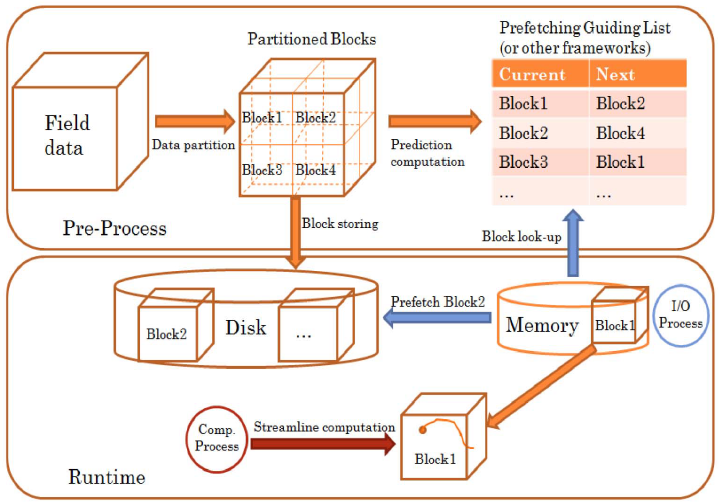
\includegraphics[width=.8\linewidth,keepaspectratio]{image/prefetch/prefetch_pipeline.png}
  \caption{
   数据预取流程图\parencite{Guo2017WL}。
 }
\label{fig:prefetch:prefetch_pipeline}
\end{figure}

数据预取的思想是在载入所需要的数据时,将之后粒子追踪可能访问到的数据也一并提前载入,
这样可以降低I/O操作次数,减少进程因为数据不在内存中而必须等待的时间,
从而提高并行粒子追踪的计算效率。
数据预取的流程图如图\ref{fig:prefetch:prefetch_pipeline}所示。
数据预取的有效性取决于对未来可能访问数据的预测准确度。
在任务并行粒子追踪的应用中,
I/O访问模式往往会被记录下来为数据预取提供依据。 
早在2005年,Rhodes等人\parencite{RhodesTBS05}就将用户访问模式作为先验知识,使用缓存和预取机制来动态提高I/O性能。图\ref{fig:prefetch:initial_prefetch}展示了其基本流程图,其中空间的预取机制成为了链接接迭代的用户访问模式和真实数据存储的重要桥梁。通过发现
迭代的用户访问模式构成的空间中访问的起点,步幅和顺序中的已有规律,可以有助于创建针对迭代进行调整的预取缓存,并进一步地根据真实的存储模型一次性的获取后续需要的文件,提升I/O的效率。接下来本文将总结近年来流场可视化并行粒子追踪过程中,利用不同流场属性特征或I/O访问模式作为先验知识来指导进行数据预取的相关工作。

\begin{figure}[!tb]
%\setlength{\abovecaptionskip}{0.05cm} 
%\setlength{\belowcaptionskip}{-0.20cm}
  \centering
  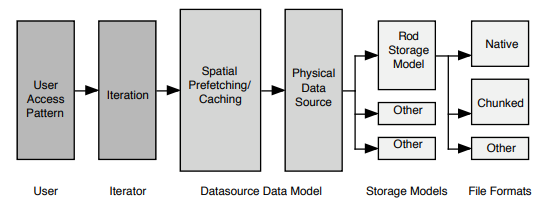
\includegraphics[width=\linewidth,keepaspectratio]{image/prefetch/initial_prefetch_patternbased.png}
  \caption{
   用户访问模式指导的数据预取框架\parencite{RhodesTBS05}。
 }
\label{fig:prefetch:initial_prefetch}
\end{figure}

% 包括访问依赖图和其他更复杂的I/O模式。

\begin{figure}[!tb]
%\setlength{\abovecaptionskip}{0.05cm} 
%\setlength{\belowcaptionskip}{-0.20cm}
  \centering
  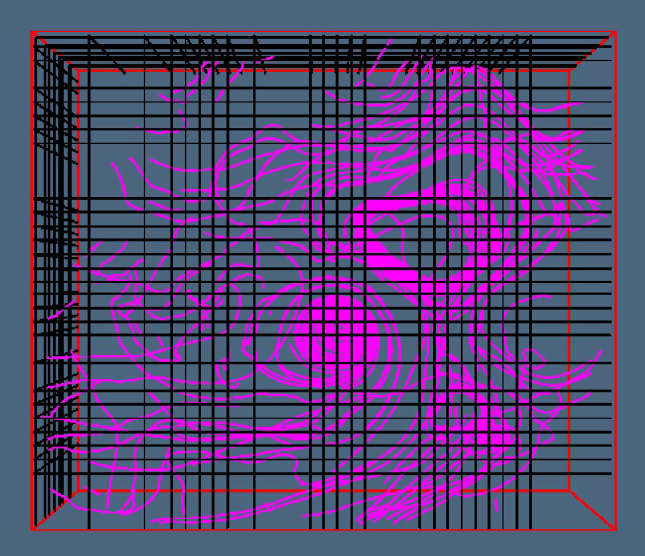
\includegraphics[width=.55\linewidth,keepaspectratio]{image/prefetch/block_partition.png}
  \caption{
   基于流场特征的自适应数据块划分方法效果示例\parencite{Guo2017WL}。其中粉色曲线为随机撒种生成的流线,黑色网格为根据此方法得到的数据块划分结果。
 }
\label{fig:prefetch:block_partition}
\end{figure}

近年来,国防科技大学海洋科学与工程研究院的Guo等人\parencite{Guo2017WL}提出了一种基于流场特征的自适应的数据块划分方法。
对于流场中较为平缓的区域,由于粒子的流向比较一致,采用不同的数据块划分策略对数据预取准确度并没有显著的影响。
而对于流场中的复杂区域,更加细粒度的划分可以更精准地预测粒子在每个数据块的流出方向。
根据上述特点,他们首先由信息熵公式计算出流场内每个区域的复杂度,然后在流场的每个维度上进行不同粒度的划分,如图\ref{fig:prefetch:block_partition}所示。
在不同数据集上的实验结果表明采用此方法可以显著提高数据块的准确预取率及有效预取率,验证了该方法的有效性。

俄亥俄州立大学的可视化小组针对流场可视化中流线和迹线等的计算,
提出了一系列基于数据访问依赖的数据预取方法\parencite{ChenXLS12,ChenNLS12}。
在预处理阶段,他们将数据划分为小块形式,
然后根据粒子追踪的数据访问关系生成数据块之间的访问依赖图(access dependency graph, ADG)。
如图\ref{fig:background:adg-1st}所示,
在访问依赖图中,每个结点代表一个数据块,
结点之间的有向边表示从一个块到另一个块的访问转移关系。
有向边的权重记录了访问转移的概率,即粒子从一个块出发到达另一个块的概率。
他们将这种数据访问依赖图用于文件布局优化,
从而在数据预取过程中帮助精确预测即将可能用到的数据块。
但是,由于访问依赖图的精度和预处理开销对数据块大小和撒种策略等比较敏感,
这些方法比较容易受到参数的影响。

\begin{figure}[!tb]
  \centering
  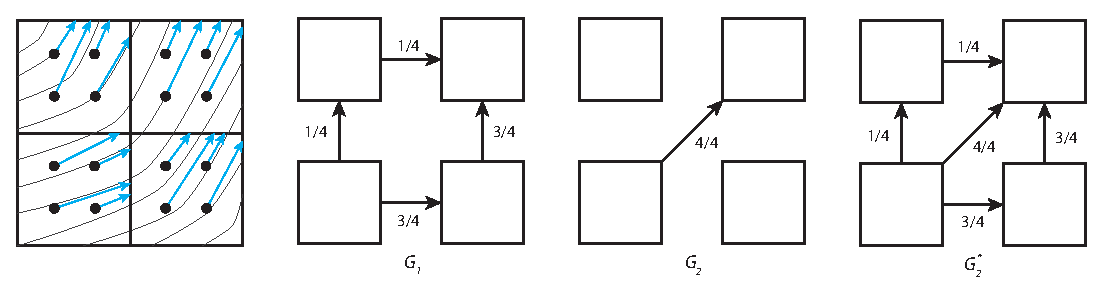
\includegraphics[width=\linewidth]{image/prefetch/adg-1st}
  \caption{
    粒子追踪过程中的访问依赖图\cite{ChenXLS12}。
    图中示例展示了粒子从起始数据块到下一个数据块($G_1$)以及继续到第三个数据块($G_2$)。
    $G_2^*$表示这两个图的混合。
  }
  \label{fig:background:adg-1st}
\end{figure}

首先,粒子的轨迹难以预测。
粒子轨迹本质上是一条积分曲线,这条曲线上的每一采样点位置的计算都依赖于前一点,
其并不像体绘制中那样,给定起始采样点和步长,就可以直接计算出后面每个采样点的位置。 
因此,即使给定了初始粒子的位置,也很难预测其轨迹的走向,
也不知道粒子会访问哪些数据,给数据的管理带来了很大的困难。

而在数据并行中,数据从外存存储组织中,按照初始的划分和分配策略,
被不同的进程载入内存,进行粒子追踪计算。
根据数据块在进程中的分布,粒子在这一过程中会在不同的进程之间交换。
由于粒子追踪计算和数据是紧密耦合的,粒子和数据在并行计算过程中的移动实际上也是紧密相关的。
数据的移动会极大地影响并行粒子追踪的I/O效率和内存使用效率。

另一方面,由于在任务并行粒子追踪过程中一般由进程按需载入数据块,
会导致频繁的I/O开销。已有的工作\parencite{ChenXLS12,ChenNLS12}中研究者们主要将数据进行小块的划分和组织,
通过一个预处理阶段,事先在流场中密集撒种统计粒子在数据块之间的访问先后关系,
生成数据块访问依赖图,然后在并行粒子追踪中使用数据预取技术,
即提前载入可能需要的数据,将I/O操作的时间“隐藏”起来,
减小I/O的开销使得粒子追踪的完成时间集中在计算上。
这里面一般是根据粒子的数据访问模式来进行数据组织,
据此设计数据的访问策略,提高I/O和内存使用效率。
数据的组织是一个预处理过程,需要预先计算数据块之间的访问模式并随原始数据存储管理,
以支持使用数据预取来减少I/O操作。其I/O效率的提高很大程度上取决于数据预取的准确率,
而数据预取的准确率又依赖于对数据的预处理,
这种预处理的复杂性往往和流场的规模和复杂性成正比,
因此目前做法的复杂度都比较高,并且需要比原始数据更大的存储组织空间。

\subsection{一阶访问依赖数据预取}

\begin{figure}[!tb]
  \centering
  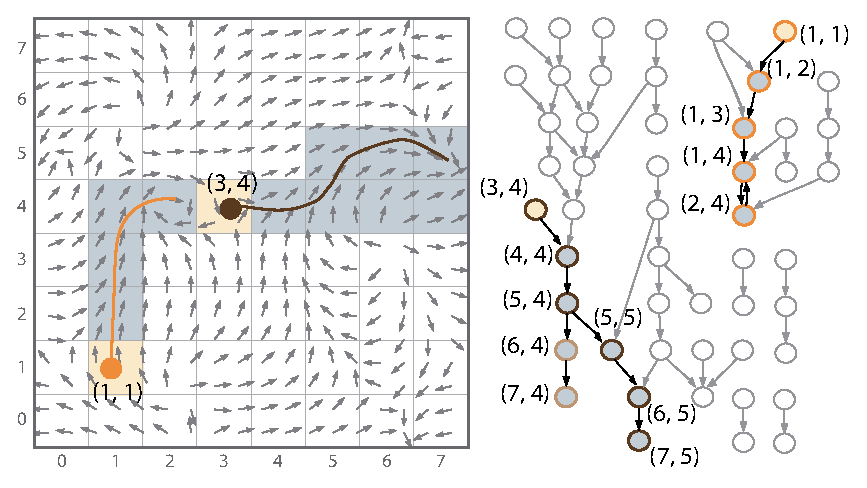
\includegraphics[width=.75\linewidth]{image/prefetch/sparse}
  \caption{
    一阶访问依赖数据预取示意图\parencite{GuoZLLYHMP14}。
  }
  \label{fig:background:sparse}
\end{figure}

在迹线计算中,数据量通常非常巨大,但是其中的迹线计算所需要的数据可能只是其中的一部分。传统的粗粒度的划分可能导致不必要的数据读取。而场线的计算随着粒子的运动具有一定的空间关系,这是由于一些模式导致的。以大规模高维数据可视化为例,对一种稀疏数据管理的方法\cite{guo2014advection}进行分析,该方法首先对数据进行“小块”的细粒度划分,并且使用基于并行键值存储的按需数据管理策略。

在并行计算迹线的过程中,该方法有效平衡了I/O带宽和数据访问请求之间的速度差距。结果表明在任意给定的资源限制下,该方法能够提高数据分析的规模,节约I/O带宽和内存的使用,提高任务并行的并行迹线计算的可扩展性。

\subsection{高阶访问依赖数据预取}

追踪大量的场线。然而,由于巨大的I/O和内存需求,场线的计算是非常昂贵的。特别是I/O开销,往往能占据整个计算时间的90\%。解决I/O负担的一个方法是将数据访问模式结合到场线计算中。数据访问模式由流场数据的特征隐式地决定,其记录了场线轨迹的数据访问情况。可以将其提取出来,并在之后的场线应用中预测数据访问。在已有的方法中,马尔可夫链被用来对数据访问模式进行建模,其思想是通过当前的数据访问预测下一个可能的数据访问。这种访问模式也被称为数据块之间的一阶访问依赖。不过,由于每个数据块可能与多个其他的数据块有访问依赖关系,因此很难得到比较准确和可靠的访问预测。

实际上,除了这种简单的一阶访问模式,在场线追踪中还存在着更为复杂的高阶访问依赖。不同之处就在于高阶访问依赖将历史的数据访问信息也考虑进去了,使之可以得到更为精确的数据访问预测。图\ref{fig:highorder_fig1}给出了一个例子。在图\ref{fig:highorder_fig1}(a)的一阶访问依赖中,数据块0与其三个邻结块1,2,3都有访问依赖关系。因此,对于一个从数据块0出发的粒子, 其下一个要经过的块有三种可能性。而在图\ref{fig:highorder_fig1}(b)的二阶访问依赖中,根据不同的历史访问,下一步要访问的数据块的可能性减小为两个,并且概率更集中。基于此,张江等人提出了一种新颖的基于高阶访问依赖的模型,以高效地计算场线,特别是非定常流场中的迹线。该方法包含两部分,首先通过迹线追踪计算出高阶访问依赖,然后将它们应用到一个并行粒子追踪框架,以证明高阶访问依赖的有效性。

\begin{figure}[!tb]
  \centering
  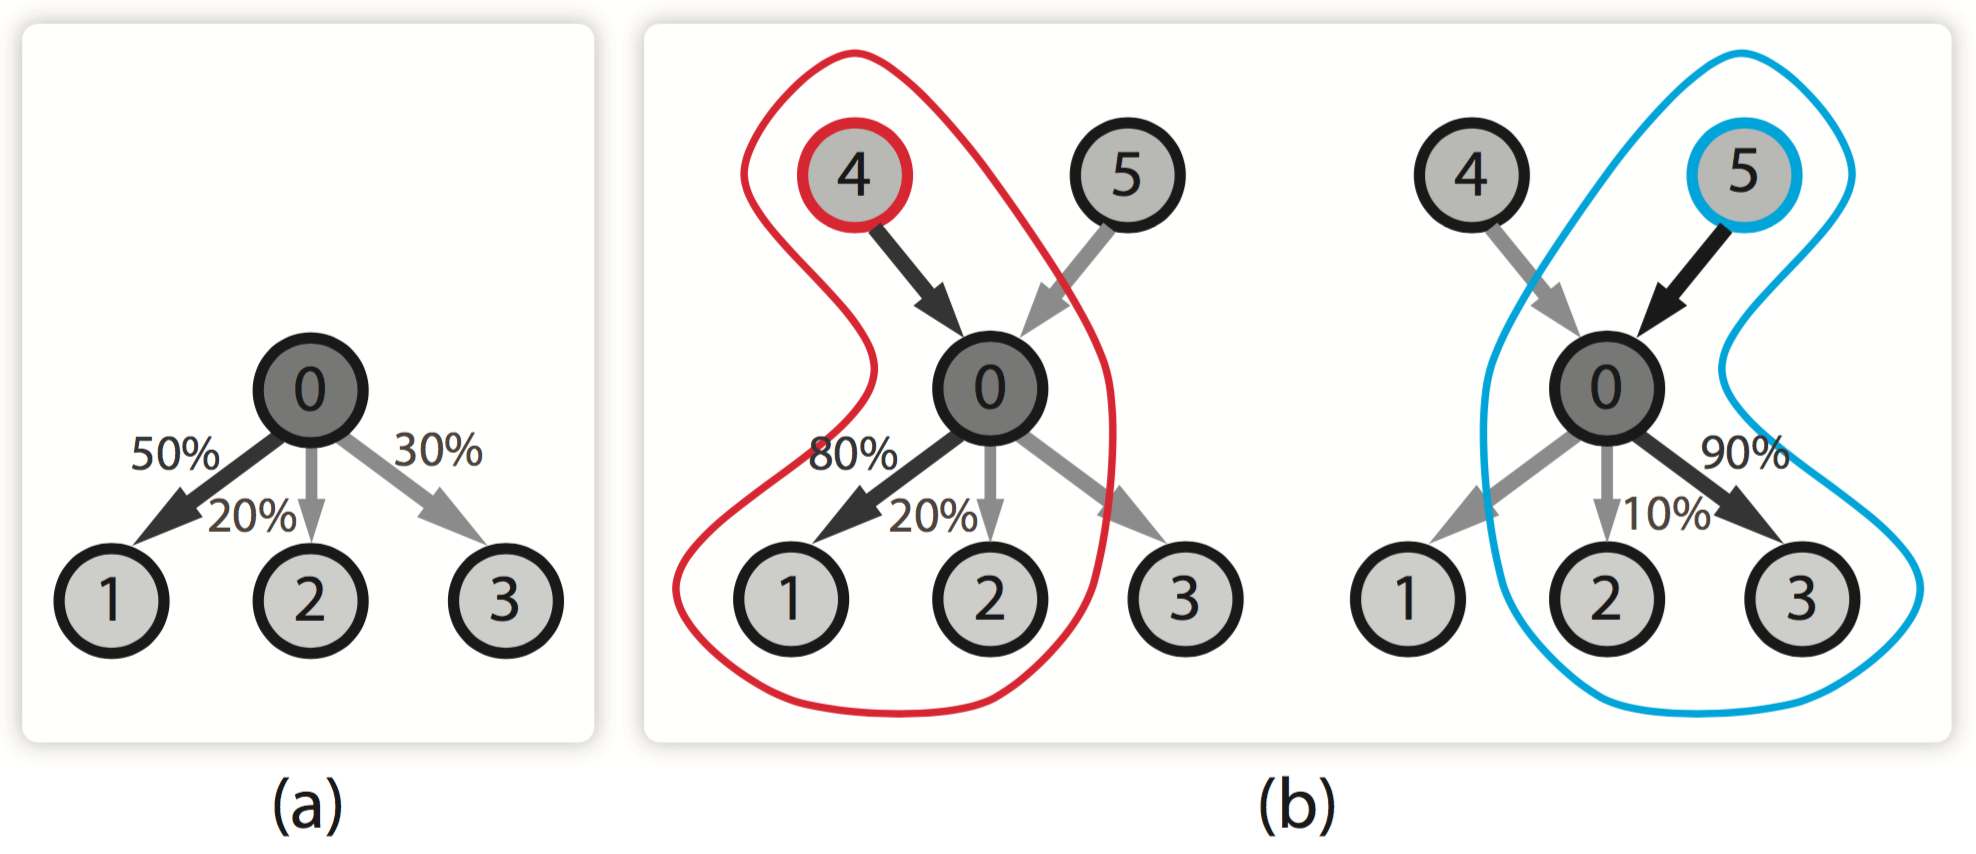
\includegraphics[width=.7\linewidth]{image/prefetch/highorder_fig1.png}
  \caption{
    使用图模型展示的(a)一阶和(b)二阶访问依赖的比较\parencite{ZhangGY16}。
  }
  \label{fig:highorder_fig1}
\end{figure}

与一阶访问依赖相比,在高阶访问依赖模型中,对下一个可能访问的数据块的预测不仅依赖于当前的数据访问,还建立在若干历史数据访问序列上。对于一个m阶访问依赖,有图\ref{fig:highorder_fig2}所示的定义。

\begin{figure}[!tb]
  \centering
  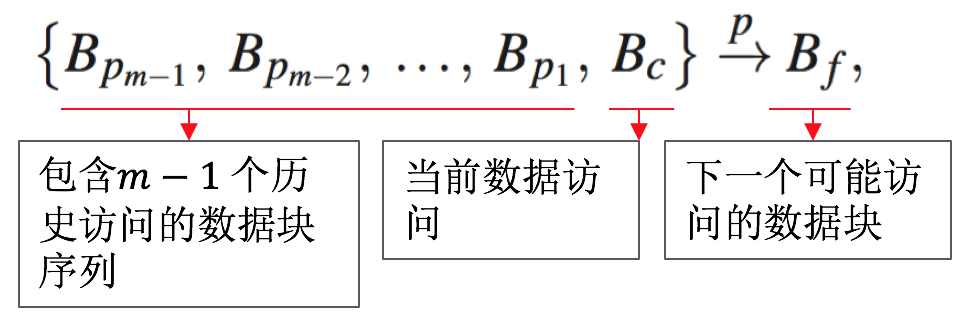
\includegraphics[width=.6\linewidth]{image/prefetch/highorder_fig2.png}
  \caption{
    m阶访问依赖的定义\parencite{ZhangGY16}。
  }
  \label{fig:highorder_fig2}
\end{figure}

为了生成高阶访问依赖,首先需要在数据全域内追踪迹线。整个数据被均匀划分为若干数据块,每个块都包含了各个维度上相等大小的范围,并且使用均匀撒种的方式在不同位置放置粒子。每个粒子从起始位置开始同时正向和反向进行追踪。对应生成的迹线分别叫做正向迹线和反向迹线。为了减小预处理开销,对于正向迹线只追踪它从起始块转移到下一个数据块,而对于反向迹线,其所经过的数据块的数量不能大于指定的阶数。实际上,始于同一个位置的正向和反向迹线可以合并成一条完整的同时包含历史和下一步访问信息的迹线。对这些合并的迹线,除去起始块,对应的反向迹线所访问的数据块可看成是历史访问信息,而对应的正向迹线访问的数据块则是即将可能的访问信息。

对于指定$m (m > 1)$阶的访问依赖,考虑历史访问的数据块序列长度为$m - 1$的所有合并迹线。因为这些迹线的历史访问信息可能仍有不同,因此将它们进一步分组。每组迹线的历史访问信息是相同的,但是下个数据访问可能是不同的。假设下一个访问的数据块共有$n$种可能性,在该方法中,每个关联相同访问历史$B_p$ (序列$B_{p_{m − 1}}, B_{p_{m − 2}}, …, B_{p_1}$的简写)和当前访问$B_c$的下一个可能的数据块$B_{f_i}$都会对应一个高阶访问依赖。其对应的访问转移概率$p_i$定义为下一个访问该数据块的所有迹线数量与访问所有可能数据块的迹线总数的比值。该过程示意图如图\ref{fig:lstm_fig2}所示。为了充分利用所生成的迹线, 计算所有阶数低于该指定值的访问依赖。这样只要一轮预处理计算,就可以满足使用不同阶访问依赖的迹线实际应用。在本节的部分,除非特别指出,所说的某高阶访问依赖都是这种“累积”的访问依赖。

\begin{figure}[!tb]
  \centering
  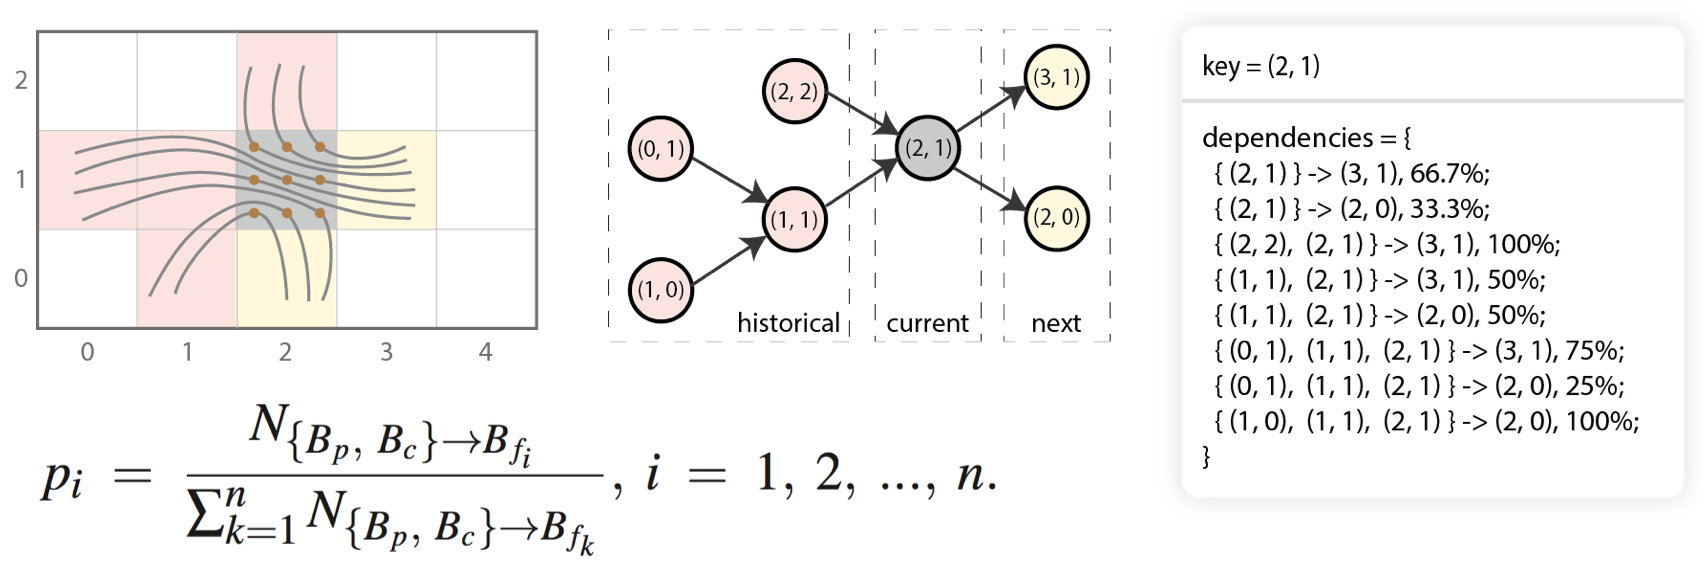
\includegraphics[width=\linewidth]{image/prefetch/highorder_fig3.png}
  \caption{
    高阶访问依赖的计算示意图\parencite{ZhangGY16}。
  }
  \label{fig:highorder_fig3}
\end{figure}


进一步将得到的高阶访问依赖应用到一个任务并行粒子追踪的框架中。数据块和其关联的高阶访问依赖是以数据项的形式进行存储。每个数据项包含三个部分:$<key, value, dependencies>$,分别表示数据块的时空索引、实际数据以及高阶访问依赖。在$dependencies$部分,对于具有相同历史访问信息的访问依赖,可以将它们重新组织,将其中下一步可能访问的数据块的$key$按照访问转移概率降序排列,这样$dependencies$里面可以看成是很多个键值对,方便之后的检索。

在运行时迹线计算过程中,使用了高阶数据预取来提高I/O效率。也就是说,当载入一个不在缓存中的数据项时,通过匹配粒子真实的历史数据访问信息和该数据项中高阶访问依赖的历史访问信息部分,得到具有最高转移概率的数据块并将其一并载入,以满足之后可能的数据访问需求。实际上,也可以通过设置预取深度来递归地预取多个深度的数据块,而在每个预取深度,也可以将多个高概率的数据块同时预取进来。图\ref{fig:highorder_fig4}展示了一个递归的预取过程。图中每个预取深度只取概率最大的数据块。

\begin{figure}[!tb]
  \centering
  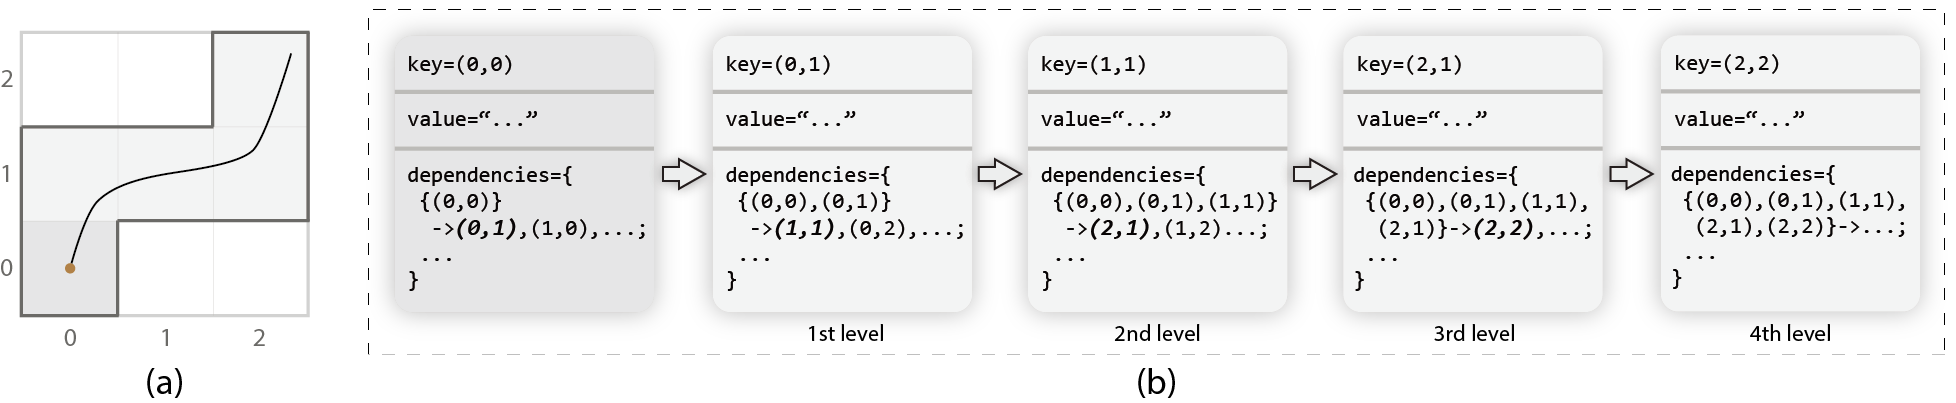
\includegraphics[width=\linewidth]{image/prefetch/highorder_fig4.png}
  \caption{
    一次性递归地预取多个数据项\parencite{ZhangGY16}。在这个例子中,预取深度设置为4,并且在每个预取深度 只预取概率最大的那个数据块。当请求块(0, 0)时,块(0, 1),(1, 1),(2, 1)和(2, 2)一个接一个地被预 测出来并被预取进内存。在每个预取深度,历史访问信息都会随之更新。
  }
  \label{fig:highorder_fig4}
\end{figure}


该方法仍然具有一定的局限性。首先是预处理开销,主要集中在迹线计算上,尽管采取了一定的策略,其代价仍然比较高,特别是对于大规模数据。因此,需要考虑更好的撒种策略。另外,合适参数的选择也是一个比较困难的问题,包括预取深度和数据块大小的设置等,虽然在该工作中都是经验指定的,但是各个参数和它们之间的联系仍然值得进一步地探究。

\subsection{深度学习支持的数据预取}
粒子追踪是流场可视化与分析里最重要的技术之一,被大量应用在场线渲染、源汇查询、有限时间李雅普诺夫指数计算等应用中。然而,在大规模流场中,对大量粒子通过粒子追踪算法计算轨迹时,由于粒子访问数据块的局部性很差,导致计算过程中有大量时间消耗在数据块的读入上。一种提高数据块访问效率的做法,就是对粒子将要访问的数据块进行预测,然后提前进行预读取,从而将读入花费隐藏在计算时间之下。这个工作\parencite{Hong2018LSTM}首次引入了深度学习模型,即基于长短期记忆 (Long Short-Term Memory, LSTM) 的模型,对粒子轨迹进行建模,从而能更为准确地预测粒子对数据块的访问,从而提高大规模粒子追踪算法的效率。

\begin{figure}[!tb]
  \centering
  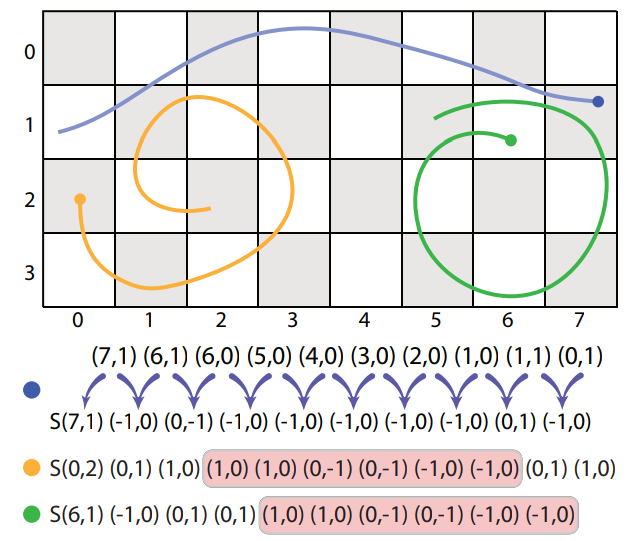
\includegraphics[width=.65\linewidth]{image/prefetch/lstm_fig1.png}
  \caption{
    粒子轨迹数据到移动序列数据的转换\parencite{Hong2018LSTM}。
  }
  \label{fig:lstm_fig1}
\end{figure}


为了将粒子轨迹转换为深度学习模型容易处理的数据,需要对其进行变换。首先,粒子轨迹的坐标序列被转化为粒子所访问数据块的序列。采用数据块而不是坐标,是已有数据预读取工作常用的做法,并且直接预测坐标容易在数据块边界附近出现错误。接下来,数据块序列被转换为相对移动的序列,即表现粒子如何在数据块之间穿行。图\ref{fig:lstm_fig1}中,以蓝色粒子为例,展示了这个转换过程,也就是相邻两个数据块的索引求差。为了保证转换后的移动序列和原本的数据块序列等价,在序列最前面加上粒子的初始数据块,并加上字母S区分。这样就完成了粒子轨迹数据的转换工作。这种转换的另一个好处是,深度学习的模型能学习到间接的访问模式。例如,图\ref{fig:lstm_fig1}中黄色、绿色粒子尽管初始数据块不同,但具有类似的旋转行为,因而在转换后的序列中具有相同的子序列。该模型能够学习到这种模式,并应用到其他粒子的行为预测中去,而已有的工作则不能。

\begin{figure}[!tb]
  \centering
  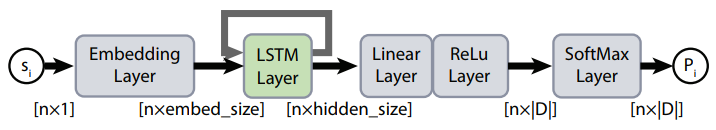
\includegraphics[width=.85\linewidth]{image/prefetch/lstm_fig2.png}
  \caption{
    基于LSTM实现的深度学习模型\parencite{Hong2018LSTM}。
  }
  \label{fig:lstm_fig2}
\end{figure}

接下来,围绕LSTM构建深度学习模型,如图\ref{fig:lstm_fig2}所示。在这里,仅介绍模型的输入输出关系,细节部分请参阅论文以及相关深度学习资料。总起来看,该输入是粒子的移动序列$s_0, s_1, …, s_{n-1}$,其中$s_0$是粒子初始数据块索引。模型输出则是对应下一步移动的概率分布$P_0,P_1,…,P_{n-1}$。最初,模型接受$s_0$为输入,对粒子的第1步进行预测,得到其在各种移动可能性上的概率分布$P_0$。接着,模型又接受$s_1$为输入,对粒子的第2步进行预测,得到其在各种移动可能性上的概率分布$P_1$。需要注意地是,由于LSTM模型的性质,$s_0$也参与到了$P_1$的生成中。以此类推,粒子每一步移动的预测均由其之前所有访问的数据块序列来决定。

为了训练这个模型,从原始流场数据中采样一些较低精度的粒子轨迹,进行数据转换,作为训练集,选择超参数进行模型训练。文中对训练集大小以及超参数的选择与预测精度的关系进行了探索。

接着,将该预训练的模型部署在GPU上,为并行粒子追踪算法提供粒子数据块访问的预测功能。粒子追踪器通过提前的数据块预取,来提高运行效率。在该性能测试中,该工作选用了三个数据集:飓风伊莎贝尔、GEOS-5大气模拟和海洋模拟数据集。测试的布种策略为局部分析和全局分析,即在局部区域密集撒种,以及在整个空间域均匀撒种。在测试中,该方法与不带预取的方法以及使用高阶访问模式\parencite{ZhangGY16}进行预取的基准方法进行对比。

相比较于不带预取的方法,该方法有很大的性能提升。而相比较于使用高阶访问模式\parencite{ZhangGY16}进行预取的方法,该方法性能略高。在其他两个数据中也有类似的表现。而在全局分析中,相比较于不带预取的方法,该方法仍然具有很大的性能提升。而相比较于使用高阶访问模式\parencite{ZhangGY16}进行预取的方法,该方法性能略低一些。

需要注意的是,尽管该方法和高阶访问模式的方法性能基本接近,但该方法所需要的额外存储要远远小于高阶访问模式的存储,并且所需要的训练样本数目也更加少。例如对于飓风伊莎贝尔数据,该模型仅占用53MB,而4阶高阶访问依赖关系需要5.7GB,6阶更是需要20GB,比原数据更大。如果要求高阶访问依赖关系仅使用与该方法相同的额外存储空间,那么它的性能将会变得非常差。另一方面,该方法仅需要100多万的粒子进行训练,而高阶访问依赖关系要数倍于此。

总的来说,该工作首次采用了深度学习的技术来解决流场可视化中的粒子追踪问题。相比于已有工作,该方法方法能取得与已有方法相当的准确率和性能提升,并且只需要极小的额外存储和训练样本。

\subsection{基于其他I/O访问模式的数据预取}
除了上面提到的比较直接的数据块之间的访问依赖关系,一些更为复杂的I/O访问模式(包括空间模式、时间模式、模式重复次数和请求数据大小等)也可以被检测并提取出来。
Byna等人\parencite{BynaCSTG08}将这种I/O访问模式记录为I/O签名(signature),结合运行时真实的数据访问,用于在MPI-IO中提供数据预取的指导。
而当I/O访问模式非常随机或不可预测时,预测预取(speculative prefetching)往往可以比较可靠地确定随后的I/O访问。
预执行(pre-execution)技术就是一个很好的例子\parencite{ChenBSTG08},其可以重叠计算和I/O访问的过程,从而减小I/O的延迟,提高并行应用程序的I/O访问性能。
这些技术也适用于并行粒子跟踪,帮助提高其计算效率。

\subsection{小结}
数据预取是通过归纳已有的任务中的固有的数据特征来预测任务接下来会访问的数据内容。
% 大规模流场可视化中的粒子追踪算法很好地展现了流线的计算过程中对不同的数据的预取的巨大优势。
% 但是由于流线本身的特征复杂,我们借助不同的方法来对其进行探索。包括基于马尔可夫链等方法计算访问依赖或采用机器学习的方法计算一些隐式的规则。
% 这一系列工作表明,对复杂的科学数据中的数据预取是一种降低计算延迟的有效手段。
数据预取可以提高数据局部性,从而在粒子追踪中获得更高的I/O效率。
但是,为了获得精确的预取精度,经常需要对数据进行复杂的预处理,例如提取数据访问依赖等I/O模式,给并行粒子追踪计算带来了额外的开销。
不仅如此,这种预处理的复杂性往往和流场的规模和复杂性成正比,也限制了数据预取方法在大规模流场数据中的使用。
数据预取比较适合于在小型台式计算机\parencite{ChenS13, ChenNLS12, VermaKP00} 或者有限计算资源下的计算平台\parencite{GuoZLLYHMP14}上进行核外(out-of-core)方式的可视化应用。

\clearpage
\section{并行计算中的负载均衡化策略}

\subsection{并行计算中的负载均衡问题}
%并行计算框架十分重要
随着当下信息技术的快速发展,科学计算产出的数据体量快速提升。与此同时,针对复杂数据本身所定义的计算任务也逐渐变得更加复杂。针对这一类大规模数据的复杂任务,并行计算的模式成为了一种十分行之有效的解决方案。并行计算指同时使用多种计算资源解决计算问题的过程,它的基本思想是用多个处理器来协同求解同一问题,即将被求解的问题分解成若干个部分,各部分均由一个独立的处理器进行计算。这可以大大提升科学计算的效率。近年来,随着高性能计算技术的发展,研究者可以更多地利用超级计算机或者并行计算集群等强大的计算资源来进行并行计算,十分有效地提升了计算结果产出的效率。

%通用并行计算框架中负载均衡问题的重要性
在并行计算的过程中,负载均衡问题显得尤为重要,需要设计精细的任务分配和调度策略,使得在并行计算的整个过程中,每个计算节点都始终被分配有较为均衡的任务量,才能最大化地利用计算资源,达到效率的最优化。如果没有较好的基于负载均衡的资源调度算法,由于初始算法的分配的不均衡和计算过程中的随机演化,负载不均衡问题时常会发生。由于计算任务本身的特性的制约,负载均衡问题也成为提升并行计算效率中的一个瓶颈所在。

%负载均衡算法简单分类
针对负载均衡的问题的解决方案通常分为静态负载均衡算法和动态负载均衡算法,不同的算法针对不同的任务场景可以高效的提升并行计算的效率。静态的负载均衡算法通常根据数据或任务的的基本特性,初始地决定任务分配和资源调度的方式,在后续的并行计算过程中不再进行后续的调度方式。这要求这一类静态负载均衡算法需要有效地预估整个并行计算过程中各个计算节点的负载,统筹兼顾全局和单个轮次,有效地帮助计算效率地提升。相对于静态负载均衡算法,动态负载均衡算法相对更加灵活有效。动态负载均衡算法不仅仅考虑初始的数据和任务特性,而是同时考虑系统的实时的状态信息决定系统负载的分配,能够适应并行计算过程中的演化,高效的实现实现系统的负载均衡。动态负载均衡算法更加复杂,因而需要考虑更多的系统状态信息,需要更多的计算资源进行处理。对于系统的负载均衡问题的处理本身就需要达成成一种平衡,即预处理代价和等待以及负载平衡后收益的权衡,需要仔细的计算和考量。相对于静态负载平衡算法,动态负载平衡算法对于整个粒子追踪的过程施加了更多的干预,因而引入了更多的预处理代价,同时使得整个过程更加复杂多变,难以预测和掌控。对于上述两种算法的使用与选择,则需要根据具体的应用场景具体分析,依据数据和任务的演化和特征,合理设计任务的调度算法,才能使得负载均衡对于整个并行计算过程的效率有较大的提升。

\subsection{流场可视化中的针对负载均衡问题的挑战}
%引入流场可视化中的并行计算任务
在科学可视化中针对大规模流场的可视化任务中,基于粒子追踪的流场可视化需要从原始数据出发生成场线。这个过程计算复杂,计算量大,而且在一些需要追踪大规模密集撒种的粒子的应用中,最后的场线规模往往比原始数据更大(甚至可能达到几个数量级的差距)。
此外,随着现代科技和计算技术的高速发展,流场数据的数据量正以几何级数的速度增长。流场本身和相关的分析任务也呈现出越来越复杂的趋势。
特别地,在一些诸如线积分卷积(line integral convolution, LIC)\parencite{CabralL93,ShenK97}、
基于有限时间李雅普诺夫指数(finite-time Lyapunov exponents, FTLE)计算的拉格朗日拟序结构(Lagrangian coherent structures, LCS)
提取\parencite{Haller2001,GarthGTH07}以及流场曲面(flow surface)计算\parencite{EdmundsLCMZW12}、
源汇查询(source-destination queries)\parencite{KendallWAPHE11}等基于场线的应用中,往往需要进行复杂的粒子追踪计算。
现实应用中单台处理机由于内存和计算能力等的限制,很难满足这种大规模粒子追踪的计算需求。
而早前研究者所使用的核外(out-of-core)技术\parencite{silva2002out,BruckschenKHJ01,EllsworthGM04}
因其I/O瓶颈在大规模流场数据中也变得越来越不适用。

%流场可视化中采用并行计算的优势
而通过采用并行计算的模式,将工作负载分布到成百上千上万甚至更多的计算节点单元(本文所提到的每个节点单元一般对应一个计算进程),由这些节点单元协作计算大规模粒子的轨迹,粒子追踪的效率会大大提高。
这也使得并行粒子追踪成为了目前基于场线的大规模流场可视化的主流趋势。

%流场可视化中采用并行计算的方法 任务/数据并行
原始数据和输入粒子经过划分,每个进程单元都会分配到一定的数据或粒子,并进行粒子追踪计算。
按照划分和分配对象的不同,并行粒子追踪主要分为两类。
一类以粒子为对象,称为任务并行(每个粒子可看成是一个任务),
每个进程分配到的是输入粒子的一部分,
数据通常会在追踪计算过程中被按需载入。
在并行粒子追踪过程中,进程各自对所负责的粒子进行追踪计算。
另一类以数据为对象,称为数据并行,其将数据划分为若干数据块,
每个进程分配到其中的一部分,输入粒子按照其初始位置所在数据块也会被分配到不同的进程中,
数据在开始追踪计算前就被载入到各进程内存中。
为了保证每个粒子的追踪能够完成,
在并行粒子追踪过程还会周期性地发生数据的移动(针对任务并行,从外存移动到内存或者在进程之间移动)
或者粒子的交换(针对数据并行,在进程之间交换)。
当所有进程完成各自的粒子追踪计算,整个并行计算过程会停止。
经过计算得到的场线会被用于对流场的可视化和分析。


% 流场可视化中负载均衡的问题
但是,不同于其他领域的并行计算,粒子追踪的并行化本身存在着比较复杂的问题。 
在进行粒子追踪过程中,粒子的运行时间也难以预测。
粒子追踪的自然终止条件一般是粒子穿出数据域的边界,或者遇到临界点等速度为零的地方,
在此之前,如果没有人为设定终止条件,粒子会一直在数据场内运动。给定一个初始粒子,粒子会在什么时候停止追踪计算难以预测,其积分步数难以确定,因此负载也难以预测。这样,对粒子的初始划分很难保证进程的负载均衡。这些问题实际上也是并行计算中的经典问题,但是粒子追踪的特性大大加重了这些问题的严重性。

\subsection{任务并行的流场可视化中的针对负载均衡问题的经典解决方案}
% 流场可视化中负载均衡的问题的解决方案
% 针对任务并行
在任务并行中,由于粒子的完成时间不同且难以预测,
初始的粒子划分和分配难以使每个进程获得均衡的负载。
当前的研究工作主要使用一些动态负载调整方法,
即在粒子追踪过程中通过动态地重新分配任务(粒子)而平衡各进程工作负载。
已有方法中,动态任务重分配算法主要分为两类,主要包括工作窃取(work stealing)和工作请求(work requesting)。
其基本思想都是当某一个工作进程完成所负责的任务时,从其他繁忙进程处转移一部分任务给该进程。这种负载状态的监听和任务的调度过程是通过一个主进程来完成的。在任务转移的过程中,数据也需要随之一同被分配,以满足粒子追踪的要求。因而实际上,这里面涉及到的也是数据的动态调度管理。不过,虽然不需要静态的数据预处理操作,这些方法因为需要专门的进程(或线程)进行调度,会带来较大的通信开销,限制了其可扩展性。
而且,在并行粒子追踪的动态过程中进行干预操作,这一操作带来的性能增益可能会被其带来的额外开销抵消掉,甚至会带来负面的影响。

基于工作窃取的算法中较为典型的工作是一种分区全局地址空间(PGAS, Partitioned Global Address Space)建模下的动态任务重分配算法\parencite{DinanLSKN09}。在该算法的指导下,每一个计算进程会维护一个双向队列来保存其即将执行的任务。当每一个进程需要执行任务时,其从队首获得其即将执行的任务信息。当一个进程处于空闲状态时,其将开始进行一种“窃取”的操作。进行“窃取”的进程首先需要从其他的进程中选择一个“受害者”进程。选取的策略存在多种,但已有工作已经证明了随机的选取方式为最优选取方式\parencite{blumofe1999scheduling}。一旦“受害者”进程被选中后,进行“窃取”的进程首先从“受害者”进程中获取元数据来确认是否他们有可以获取的工作任务。如果确认存在可以“窃取”的任务,则“受害者”进程维护的任务队列会被锁定,“窃取”任务的进程则会将多个任务从受害者进程的维护的任务队列的尾部将任务转移给自己,转移的任务数量可以是一个或多个。如果受害者进程没有多余的任务可供“窃取”,则进行“窃取”操作的进程再一次随机的选择一个新的“受害者”进程,并重复这一操作,直到获取了可以执行的任务亦或者是其检测到了全局完成的信号。图\ref{fig:loadbalance:workstealing}展示了基于上述流程总结的算法伪代码。

\begin{figure}[!tb]
%\setlength{\abovecaptionskip}{0.05cm} 
%\setlength{\belowcaptionskip}{-0.20cm}
  \centering
  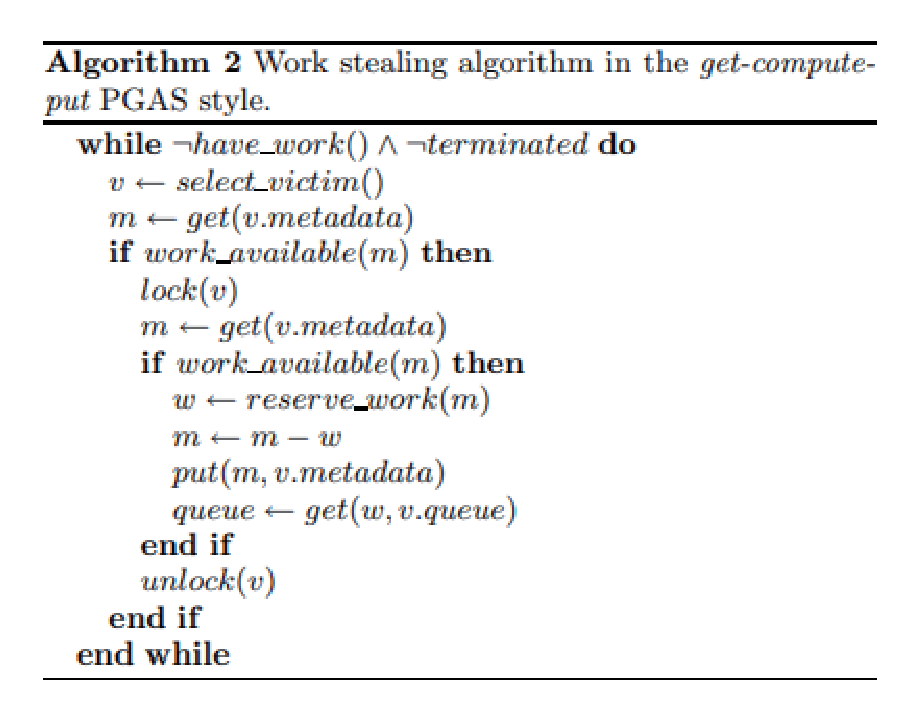
\includegraphics[width=0.7\linewidth,keepaspectratio]{image/loadbalance/PGAS_workstealing.eps}
  \caption{
    分区全局地址空间建模下的基于工作窃取的动态任务重分配算法\parencite{DinanLSKN09}。
 }
\label{fig:loadbalance:workstealing}
\end{figure}

基于上述方式的动态任务重分配算法可以灵活地适用于多种流场可视化应用,并基于MPI消息通信的并行框架可以带来有效地实现。俄亥俄州立大学的可视化小组针对流场可视化中的流面绘制计算过程就施加了基于工作窃取的算法以解决并行计算中的负载均衡问题\parencite{LuSP14}。其基本算法如图\ref{fig:loadbalance:workstealing_mpi}所示。

\begin{figure}[!tb]
%\setlength{\abovecaptionskip}{0.05cm} 
%\setlength{\belowcaptionskip}{-0.20cm}
  \centering
  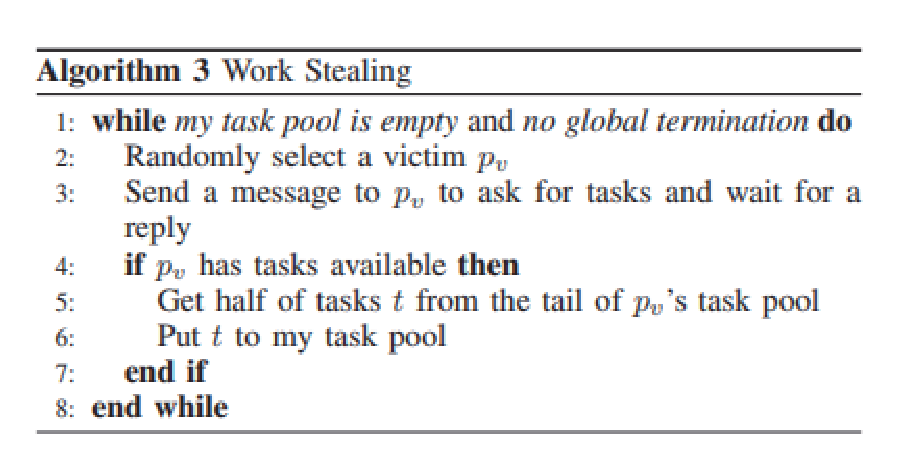
\includegraphics[width=0.7\linewidth,keepaspectratio]{image/loadbalance/streamline_workstealing.eps}
  \caption{
    基于MPI并行框架下基于工作窃取的动态任务重分配算法\parencite{LuSP14}。
 }
\label{fig:loadbalance:workstealing_mpi}
\end{figure}

基于工作请求的算法与基于工作窃取的算法原理相似。不同于基于工作窃取的算法中多个工作进程之间直接进行通信,并转移工作负载和对应的数据,基于工作请求的算法将不同进程根据其不同职责划分为工作进程和监管者进程两类\parencite{MullerCHG13}。算法之所以进行上述的改良是因为试图进行“窃取”操作的进程与“受害者”进程之间试图建立通信时,受害者进程可能处于计算任务的状态而导致长时间难以回应,继而空闲进程需要长时间才能获取分担其他进程的任务。在基于工作请求的算法中,工作进程负责数据I/O和粒子追踪积分计算,当其完成其任务队列中的所有任务时,则向监管者进程发出工作需求申请,监管者进程收到工作需求申请后,若其持有未完成的工作任务,则将半数的任务递交给提交该申请的工作进程。当监管者进程发现其持有的工作任务均被派出,则同样随机选取一个“受害者”进程并向其请求一部分任务。整个过程中,监管者进程起到了调度者的角色,减少了与工作进程通信的次数,减少了等待的时间,同时使得全局的通信模式更加合理。其基本算法如图\ref{fig:loadbalance:workrequesting}所示。

\begin{figure}[!tb]
%\setlength{\abovecaptionskip}{0.05cm} 
%\setlength{\belowcaptionskip}{-0.20cm}
  \centering
  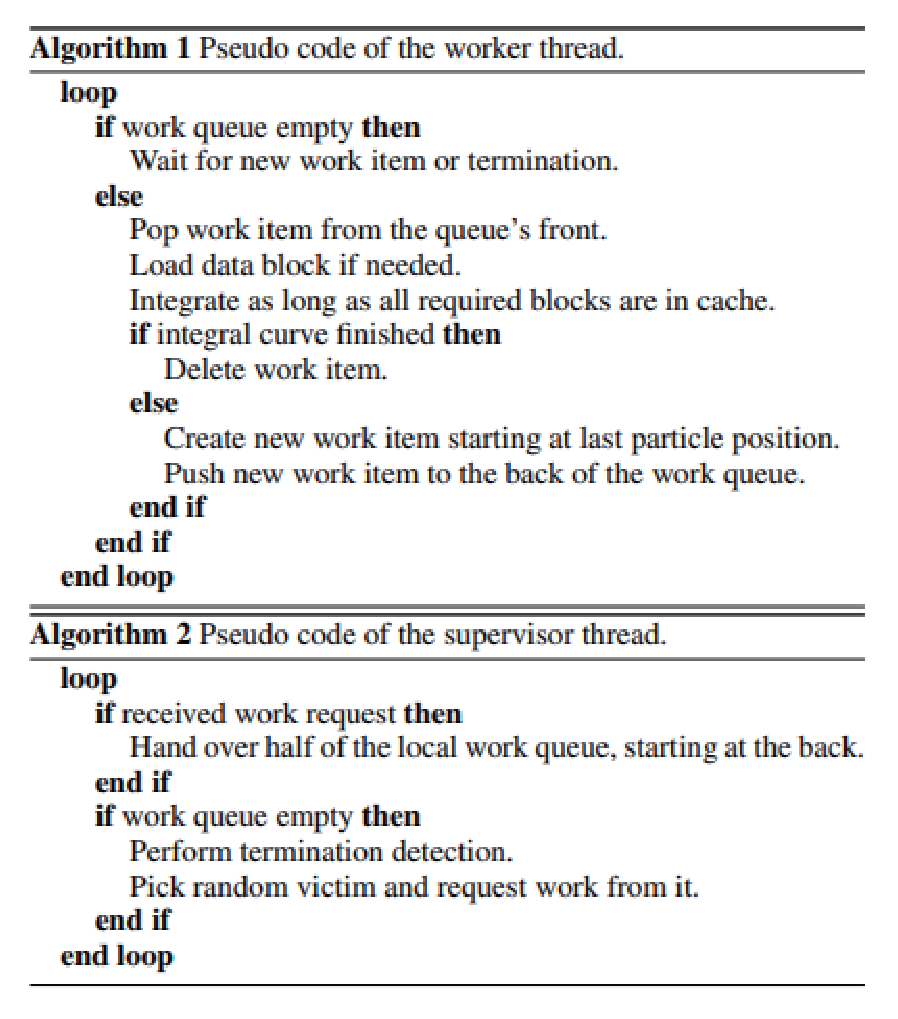
\includegraphics[width=0.8\linewidth,keepaspectratio]{image/loadbalance/workrequesting.eps}
  \caption{
    基于工作请求的动态任务重分配算法\parencite{MullerCHG13}
 }
\label{fig:loadbalance:workrequesting}
\end{figure}

北京大学可视化与可视分析小组提出了另一种针对任务并行的动态负载平衡的算法\parencite{ZhangGHYP18}。具体的说,其使用基于k-d结构的数据划分管理策略,通过周期性地进行k-d树的分解来尽量均匀地对粒子进行重新分配,从而达到负载均衡的目的。

\begin{figure}[!tb]
%\setlength{\abovecaptionskip}{0.05cm} 
%\setlength{\belowcaptionskip}{-0.3cm}
  \centering
  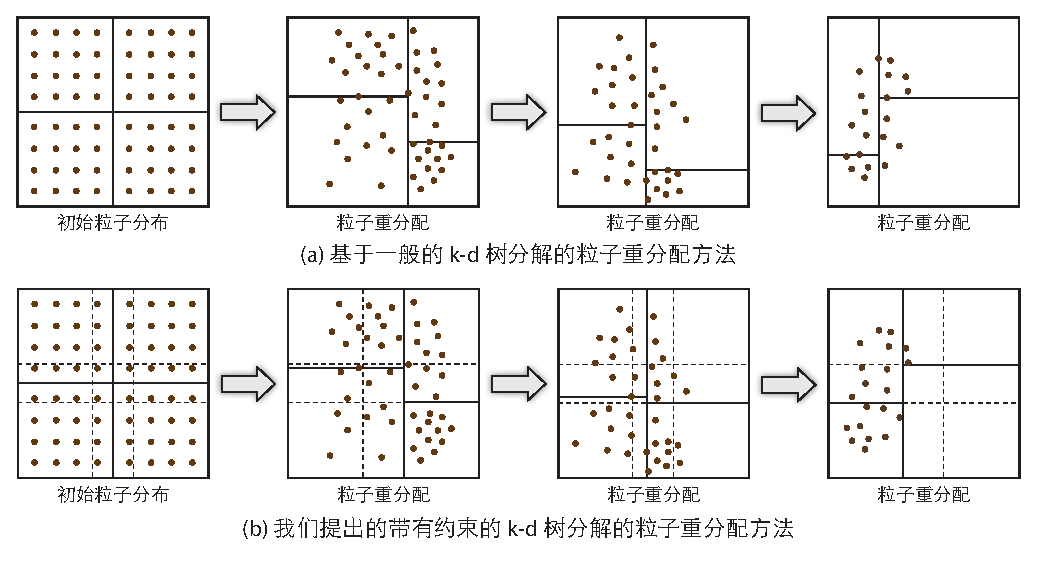
\includegraphics[width=0.99\linewidth]{image/loadbalance/basic-idea}
  \caption{
    基于一般k-d树分解的和新的带有约束的k-d树分解的粒子重分配示例。\parencite{ZhangGHYP18}
    在图(a)和(b)中,实线表示的切分线将粒子尽量划分均匀。
    图(b)中的虚线展示了由ghost层组成的数据重叠区域,其限制了切分线的位置。
  }
  \label{fig:kdtree:basic-idea}
\end{figure}

在该方法中,每个进程被分配到(1)一个静态划分的数据块,
该数据块与其相邻的被分配到其他进程的数据块会产生部分重叠;
(2)一个动态确定的k-d树叶结点,
该结点的范围受到对应数据块的几何约束,用于限制活动的粒子的重分配。
在给定的数据块重叠程度下,该方法可以最大可能地平衡各进程中粒子的数目。
与其他针对并行粒子追踪的负载平衡算法相比,
该方法不进行任何的预先分析,不使用基于流场特性的任何启发,
不对初始粒子种子的分布做任何假设,
在运行期间不移动任何数据块,并且不需要任何主进程进行任务的调度。

\begin{figure}[H]
%\setlength{\abovecaptionskip}{0.05cm} 
%\setlength{\belowcaptionskip}{-0.3cm}
  \centering
  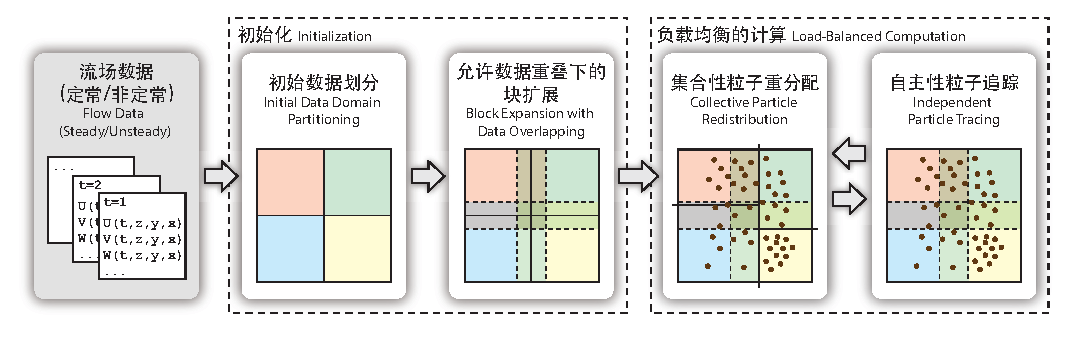
\includegraphics[width=\linewidth,keepaspectratio]{image/loadbalance/workflow_kdtree.eps}
  \caption{
    动态负载平衡方法的工作流程。\parencite{ZhangGHYP18}
    在初始化阶段原始数据首先被划分为块。
    通过增加ghost层,这些块会被扩展,使得在内存限制下与其他块有最大的数据重叠。
    在运行时阶段,集合性粒子重分配和自主性粒子追踪会被轮流执行,以动态地达到负载平衡。
  }
  \label{fig:kdtree:workflow}
\end{figure}

该方法首先对数据块和粒子进行初始化。

{\bf 数据域划分}\quad 算法通过迭代地切分数据域的每个维度来划分输入数据;
数据维度被划分的顺序与k-d树分解的一致。
不失一般性,该方法假定进程数$n$是2的幂(如果不是的话算法也可以根据其素数分解来划分每个维度)。
举例来说,在3D数据中,算法在$x$轴上找到一个位置将数据域均匀划分为两个块,
然后将这两个块的每一个再沿着$y$轴划分成两个块,然后对每一个块再沿着$z$轴划分。
$z$轴之后,下一个划分的维度又是$x$轴。
该过程一直迭代下去,直到数据块的数目等于$n$。此时每个进程可以拥有一个数据块。 数据域划分的结果是得到$n$个无重叠、相等大小、轴对齐的数据块。

{\bf 数据块扩展}\quad 该方法通过在数据块上加上ghost层来最大化块之间的数据重叠。
如图\ref{fig:kdtree:ghost}所示,每个块在所有维度上被扩展,并因此与邻近的块产生数据重叠。
块扩展使得k-d树分解的切平面可以在这个重叠区域内进行切分,其详细介绍会在下节解释。
数据块能够扩展的厚度由进程的可用内存所决定。
在内存可以容纳下整个数据的极端情况下,每个进程保存了完整的数据副本。

{\bf 数据块I/O读取}\quad 该方法并行地载入扩展后的数据块,使得每个进程将其所负责的那一部分数据读取进内存。
并行I/O由BIL(block I/O layer)\parencite{KendallHPLR11}库所实现,
其本质上是使用并行I/O以可扩展的方式来读取扩展后的数据块。

{\bf 粒子初始化}\quad 该方法载入输入粒子并且将它们在不同的进程上进行分布。
每个粒子被分配给"核心"区域(即除去ghost层)包含该粒子的数据块。
\begin{figure}[!tb]
%\setlength{\abovecaptionskip}{0.05cm} 
%\setlength{\belowcaptionskip}{-0.3cm}
  \centering
  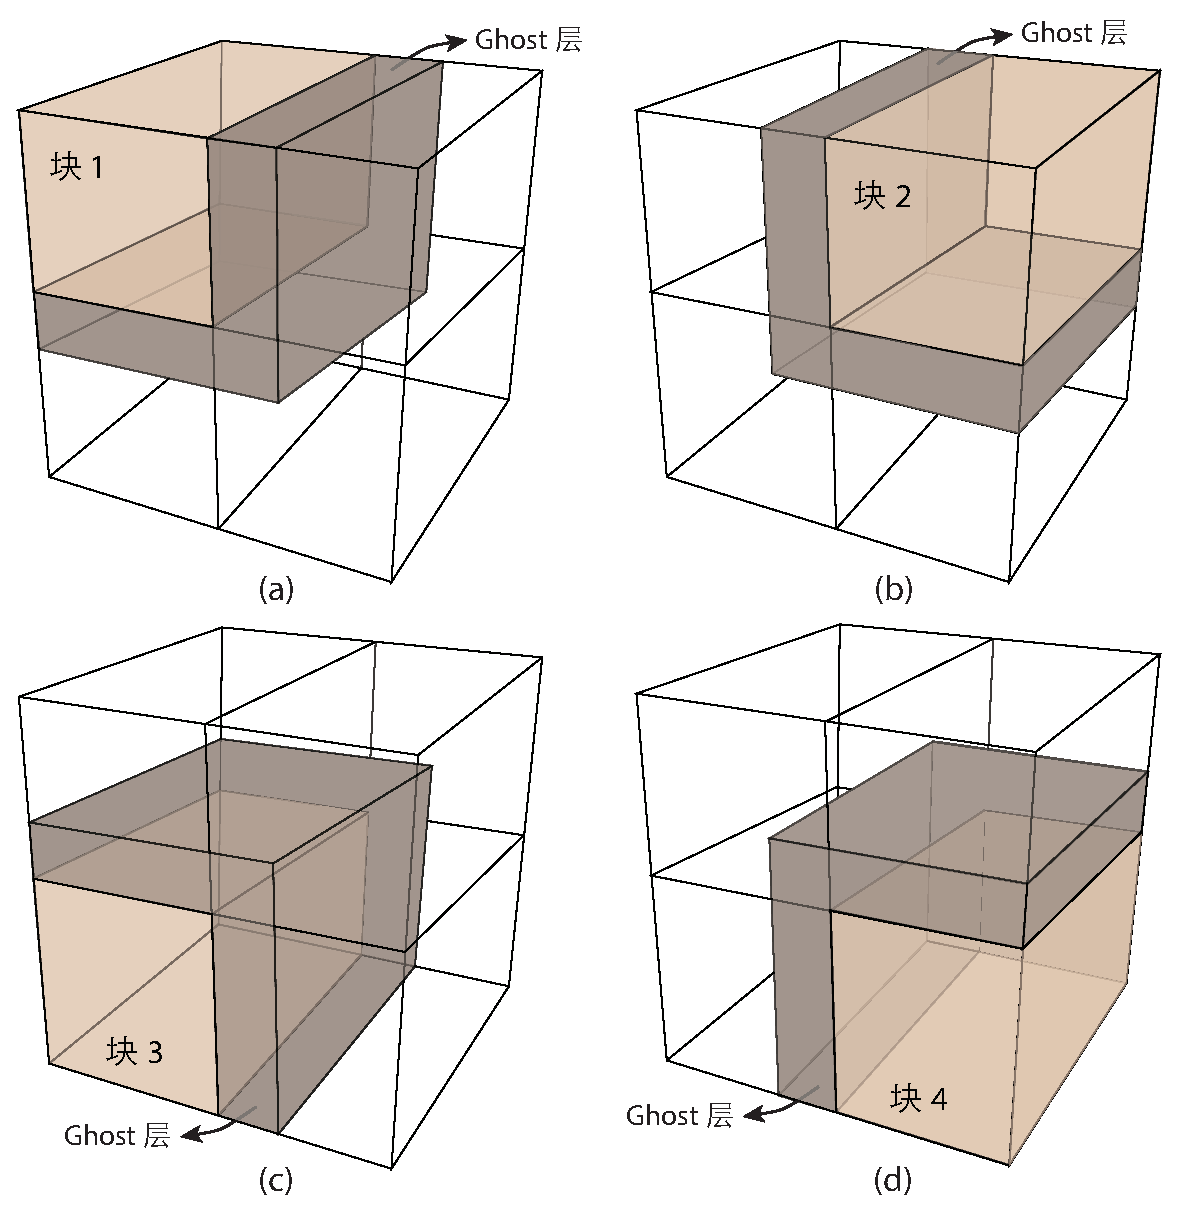
\includegraphics[width=0.6\linewidth]{image/loadbalance/ghost}
  \caption{四个经过扩展的3D数据块划分的示例。\parencite{ZhangGHYP18}}
  \label{fig:kdtree:ghost}
\end{figure}

该算法循环遍历每个维度来划分数据域。
对于每个维度,算法试图找到一个可以均匀切分粒子的轴对齐的中间平面。
如果该平面不在两个相邻数据块的重叠区域之内,则
在重叠区域的两个边界中选择可以尽可能平衡粒子数目的那个边界作为切平面的位置。

该方法重新设计了分布式k-d树分解算法\parencite{MorozovP16},使得其切分平面可以被限制在指定区域。
该过程是一个迭代过程,每次迭代都包含两个关键部分:中间值选取和粒子交换。
初始时,该方法将所有的进程看成一组。
在第一次迭代中,每个进程统计其粒子的局部直方图,并将其发送到组内的指定根进程进行聚集。
之后根进程根据上面所讲的规则在第一个坐标上
找到一个位于数据块重叠区域内的中间平面(以对应坐标上的值表示),
再将其广播给组内所有其他的进程。
该中间值将所有粒子分成两部分,使得在几何限制下每部分的粒子数目尽量一致。
对于粒子交换,进程会进一步被分为两个小组,
来自其中一个小组的每个进程从另一个小组中选择一个对应进程来交换粒子,
以便一半的进程接收到在第一个坐标上的的投影值小于所选中间值的所有粒子,
而另一半则接收其投影值超过该中间值的所有粒子。
给定$n$个进程,通过循环切分坐标,该算法会在每一个进程小组内重复,
直到执行完$\log_{2}n$次迭代。

\begin{algorithm}
\caption{trace\_particles(local\_block, local\_particles)} 
\label{alg:kdtree:trace}
\begin{algorithmic}
%\Function{trace\_particles}{unfinished\_particles[]}
 \For {each particle $p$ in local\_particles}
   \State $N \leftarrow$ 0
   \While {$N \leqslant N_{max}$}
     \State $p \leftarrow$ RK4(local\_block, $p$)
     \Comment{\textit{使用RK4数值积分计算粒子追踪的一步}}
     \State {$N \leftarrow N + 1$}
     \If {check\_finish($p$)} 
     \Comment{\textit{检查粒子是否离开数据域或到达临界点}}
       \State local\_particles.remove($p$)
       \State finish\_particle($p$)
     \ElsIf {!local\_block.contains($p$)}
       \Comment{\textit{检查粒子是否离开对应进程负责的数据块}}
       \State break
     \EndIf
    \EndWhile
  \EndFor
%\EndFunction
\end{algorithmic}
\end{algorithm}

带有约束的k-d树分解能够将粒子尽量划分均匀,
同时确保粒子被限制在相应进程的数据块范围内。
较厚的ghost层可以更均匀地划分粒子,从而获得更好的负载均衡性。
每个进程自主性地对其数据块中的粒子进行独立的追踪计算,并且不与其他进程产生通信,如算法\ref{alg:kdtree:trace}所示。
在每轮追踪之后,粒子要么完成追踪,要么还需要继续计算。
如果粒子离开数据域,或者碰到速度为零的关键点,再或者达到可视化和分析算法所需要的最大的积分步数,
则该粒子被标记为已完成,否则为未完成。
未完成粒子会在下一轮被重分配,其过程如上一小节所讲。

该算法限制每轮一个粒子可以被追踪的最大的积分步数($N_{max}$)。
这也是该方法中的一个重要的参数,因为它间接地指定了粒子重分配的频率。
如果重分配操作执行地非常频繁,负载会更均衡,但是重分配本身总的代价也会更高。
相反,如果重分配执行的间隔比较大,该方法就不能很好地平衡进程的负载。


\subsection{数据并行的流场可视化中的针对负载均衡问题的经典解决方案}
% 流场可视化中负载均衡的问题的解决方案概览
% 针对数据并行

在数据并行中,为了使进程在粒子追踪过程中的负载相近,经常需要在初始时设 计高效的数据划分和分配策略,这一类方法被称为静态数据划分方法。由于粒子是在数据域内进行追踪,每个数据块实际上 记录了一定数量的负载。我们需要将数据划分为块,使得每个进程可以被分配到包含 相近负载的一个或多个数据块。早先的一些数据划分方法包括八叉树、k-d树、空间填 充曲线以及针对非结构网格数据的自适应网格优化等,以支持在体绘制等领域应用中 对数据进行快速检索,提高数据访问效率。

由于粒子轨迹的难以预测性和流场的复杂性,很难保证每个进程在数据分配后具有相同的工作负载。特别地,当流场包含比较强烈的局部特征(如漩涡等),
或者种子只在某些局部区域密集分布时,可能会导致进程间的负载严重失衡,降低可扩展性。因此,针对数据并行的数据管理方法旨在使用好的数据划分和分配策略来解决这些问题。我们需要将流场特征结合到划分过程中。数据的划分和分配策略对于在并行粒子追踪中获得静态负载均衡性非常重要。

我们将已有方法分为两类,即根据网格规则的数据划分和基于流场特征的不规则划分。 按照网格规则划分是一种常见的数据划分方法。在空间范围内,整个流场被均匀划分为若干个数据块,不同数据块的每个维度都包含了对应等长的一定范围。因此数据块的划分粒度是一个能够影响性能的参数,往往需要根据粒子的分布决定。

假设一共有n个进程,数据被划分为m个块,最直接的划分方法是轮转法\parencite{PeterkaRNLSKH11},即将数据块按照轮转的顺序分配给每个进程。
也即是,第i个进程被分配到第${b_{i}, b_{i+m/n}, b_{i+2∗m/n}, . . . }$这些数据 块。这种轮转方法可以确保每个进程被分到相等数量的数据块,并且这些块的空间位 置不连续,因而在实际应用中非常普遍。同时可以通过引入一定的随机性,提高了每个进程持有比较均匀粒子追踪步数的数据块的概率。

虽然这只能在一定程度上提高负载均衡性,但好处是不需要任何其他的开销。
俄亥俄州立大学的可视化小组在对于在大规模矢量场中计算多个FTLE值的流场可视化应用中同样采用了轮转法进行数据块的划分\parencite{NouanesengsyLLSP12}。
为了最大限度利用进程资源,该工作同时采用了一种并发处理多个时间间隔的流水线方法。如上图所示,所有进程组被分配到一定数量的时间间隔。在粒子平移的开始阶段,所有进程组会载入其第一个时间间隔并开始粒子追踪。当粒子到达块边界时,它会被送到包含该块的进程中继续平移。当所有可能的粒子超出了该时间间隔范围后,对应的进程组会载入下一个时间间隔,直至所有的时间间隔都被载入。

\begin{figure}[!tb]
%\setlength{\abovecaptionskip}{0.05cm} 
%\setlength{\belowcaptionskip}{-0.20cm}
  \centering
  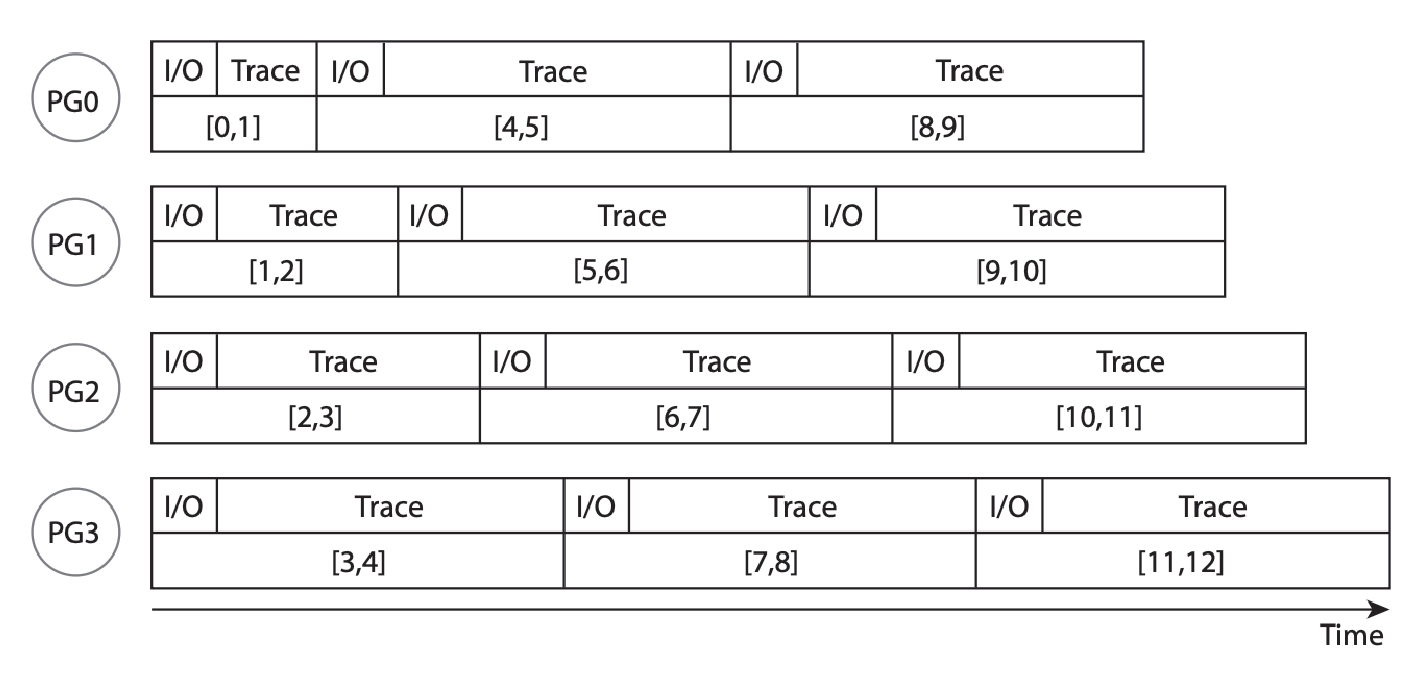
\includegraphics[width=\linewidth,keepaspectratio]{image/loadbalance/Round-robin.eps}
  \caption{
    基于轮转法的数据重划分算法\parencite{NouanesengsyLLSP12}
 }
\label{fig:loadbalance:round-robin}
\end{figure}

而为了更进一步地解决计算负载不平衡的瓶颈,
研究者也使用了负载感知方法\parencite{NouanesengsyLS11},静态评估每个数据块的负载,并据此对数据块进行分配。该方法需要通过一个预处理阶段得到数据块之间的访问依赖关系,再结合初始粒子的数量和分布去预估每个数据块的负载,然后使用划分算法进行划分。该方法将数据块的划分看作可重叠的划分任务,每一个进程每轮被分配数据块的同样的一定占比,即处理该数据块中一定比例的粒子,进行逐块(Block-wise)的粒子追踪。该优化的任务目标是最小化粒子追踪整个过程中多个进程之间的负载差异之和。该方法最终采用参数最优化的解析计算方式,计算得出每一个数据块分配给各个进程的占比参数,并据此为划分策略进行数据块的划分。每个进程只负责重复数据块中一部分的粒子追踪的工作量,但总的负载比较均等。不过,由于需要比较复杂的预处理过程,该方法只适合于种子数量很多的情况,种子数量比较少时并不划算。此外,该负载静态评估的方法也需要提前知道初始粒子的分布。
图\ref{fig:loadbalance:static_partition}给出了该工作的一个划分过程示意图。

\begin{figure}[!tb]
%\setlength{\abovecaptionskip}{0.05cm} 
%\setlength{\belowcaptionskip}{-0.20cm}
  \centering
  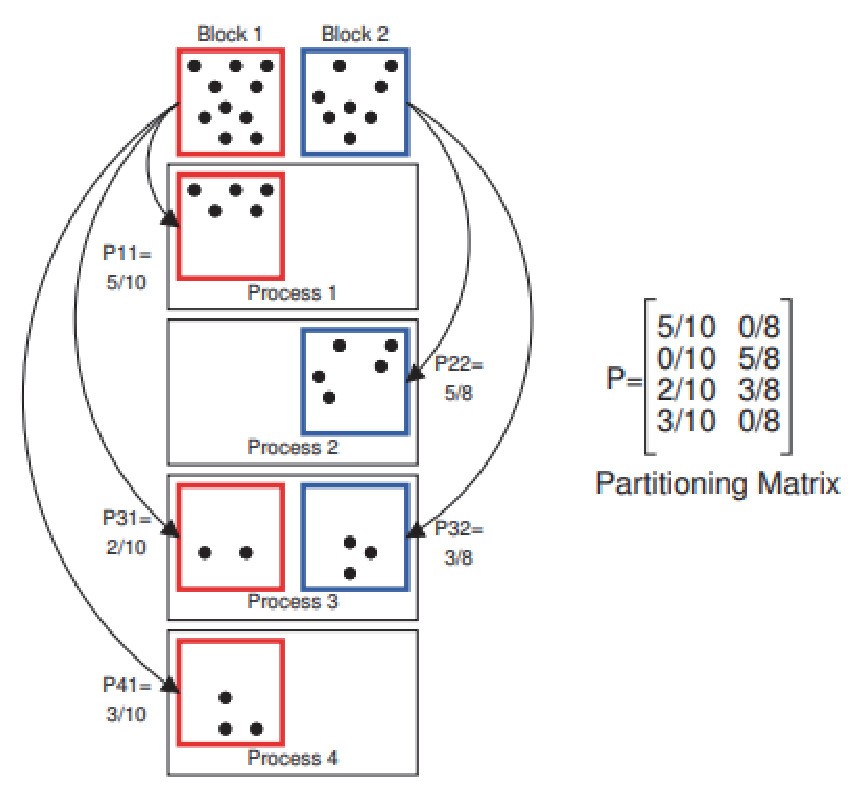
\includegraphics[width=.7\linewidth,keepaspectratio]{image/loadbalance/static_partition.eps}
  \caption{
    基于负载感知的静态数据重划分方法\parencite{NouanesengsyLS11}。
 }
\label{fig:loadbalance:static_partition}
\end{figure}

按照网格规则划分虽然操作比较简单,但是没有考虑流场数据本身的特点,是一种粗粒度的划分。对于一些特点非常明显的流场而言,基于这些流场特征的不规则划分往往更高效。如图所示,图\ref{fig:loadbalance:flowdirection}中小圆圈表示种子点,黑色实线表示流场的流向。红色虚线是按照网格规则划分的结果,这种划分方法会导致场线频繁地进入不同进程负责的数据块,造成额外的通信开销。不仅如此,按照图上的种子分布,粒子追踪过程中会有一部分进程经常处于空闲状态,造成负载不均衡的现象。因此,这时候我们往往需要考虑另一类数据划分方法,即不规则的数据划分。图\ref{fig:loadbalance:flowdirection}中蓝色虚线展示了一种根据流场方向的数据划分方法\parencite{ChenF08}。这种方法在划分的过程中考虑了种子的分布和诸如漩涡等流场的局部特征,在保证进程负载均衡的情况下,尽量使得每个粒子的追踪计算始终由同一个进程或很少的进程负责完成,减少了进程通信和同步带来的巨大开销。

\begin{figure}[!tb]
  \centering
  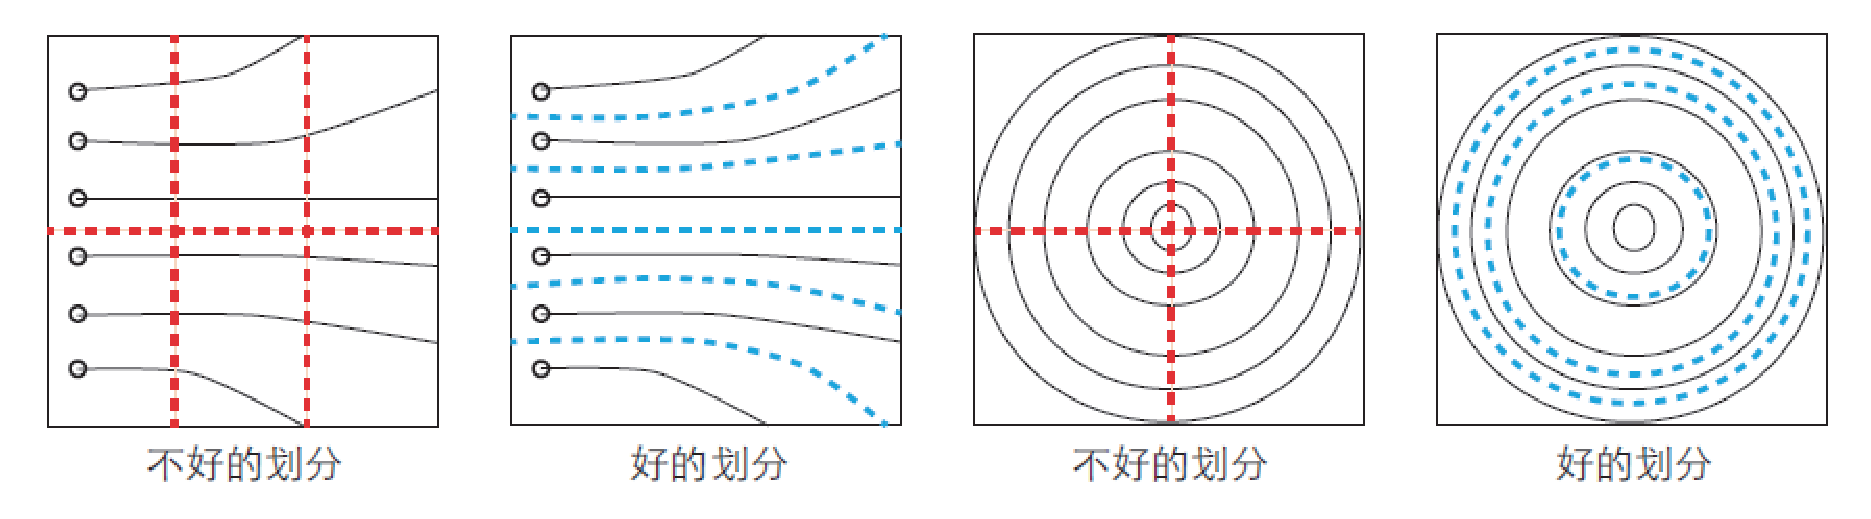
\includegraphics[width=.9\linewidth,keepaspectratio]{image/loadbalance/flowdirection.eps}
  \caption{
    规则划分和按照流场方向不规则划分的比较\parencite{ChenF08}。
 }
\label{fig:loadbalance:flowdirection}
\end{figure}

另一种不规则的划分是利用层次聚类进行自适应网格区域划分\parencite{YuWM07}。如图\ref{fig:loadbalance:hierarchical_partition}所示,数据首先被分解成单位网格,即最小的簇,然后具有类似模式的相邻网格会被两两合并,自下而上迭代地形成二叉树的层次结构。二叉树的深度实际上反映了流场特征的粒度。在数据划分时,可以根据该结构灵活选择不同层次中的簇(图中蓝点所示),评估其对应区域的负载,然后再分配给不同的进程。这两种不规则划分的方法都依赖于流场特征分析,但是在分布式环境中如何准确定义特征,也是一个新的挑战。而且,数据预处理和算法中需要预知粒子分布也带来了额外的计算负担。

\begin{figure}[!tb]
  \centering
  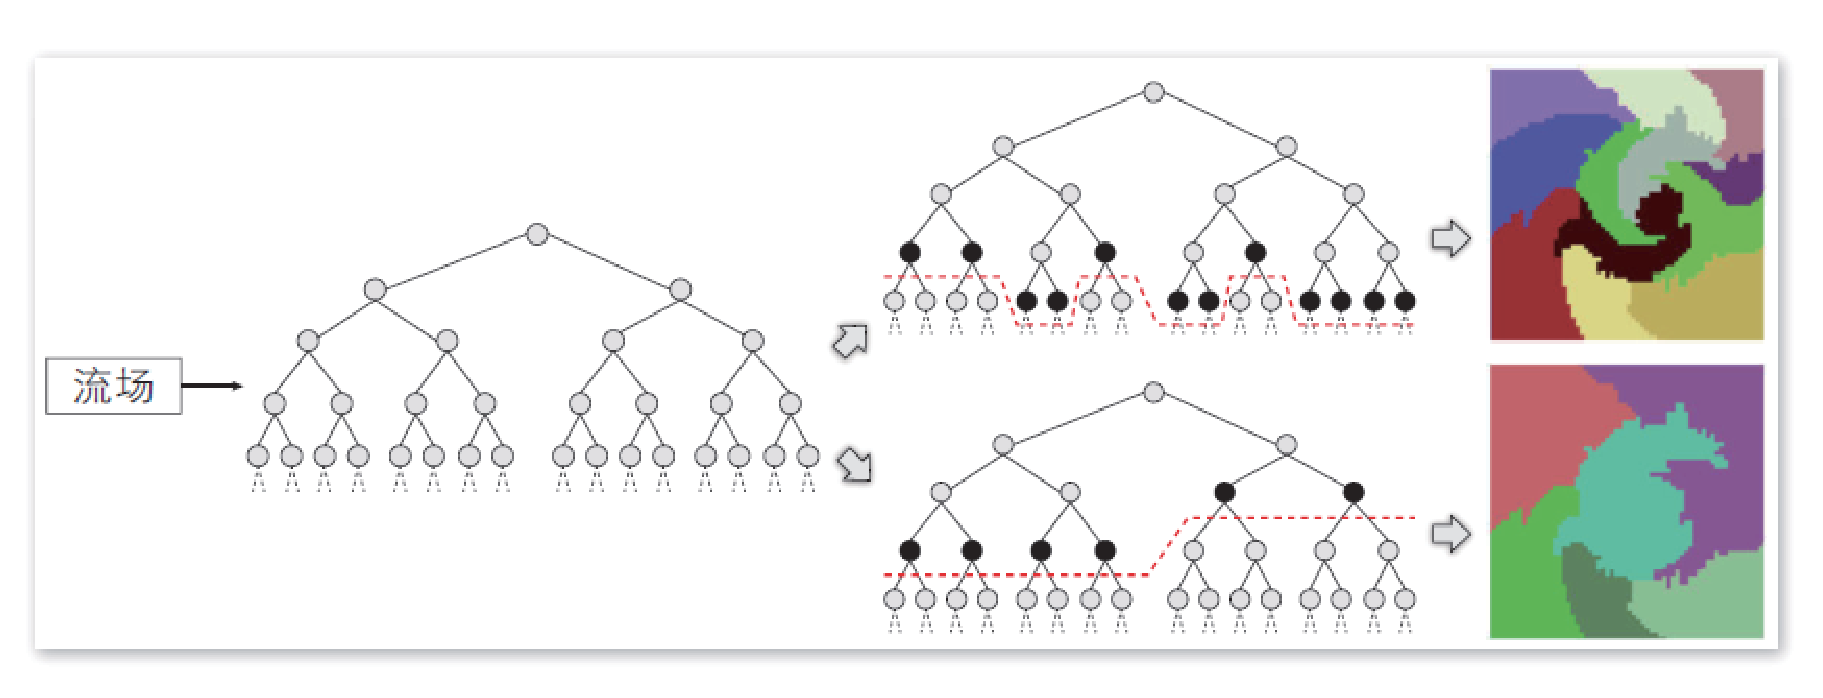
\includegraphics[width=\linewidth,keepaspectratio]{image/loadbalance/hierarchical_partition.eps}
  \caption{
    基于自适应层次聚类的数据划分\parencite{YuWM07}。
 }
\label{fig:loadbalance:hierarchical_partition}
\end{figure}

为了克服静态数据划分和分配的缺点,研究者们也提出了一些动态负载平衡的方 法。与静态方法相反,动态方法旨在粒子追踪过程中对数据进行动态划 分并将划分的数据块重新分配给各个进程,以达到负载平衡的目的。
数据重划分算法主要包含几何和拓扑两类。
几何方法根据划分对象的几何坐标进行划分,
包括递归坐标二分(recursive coordinate bisection, RCB)\parencite{BergerB87},
递归惯性二分(recursive inertial bisection, RIB)\parencite{Simon91},
以及空间填充曲线(space-filling curves)\parencite{PilkingtonB94}等算法,
而拓扑方法则需要先构造分区对象的拓扑结构,将其转化为图\parencite{GeorgeV96}
或者超图\parencite{CatalyurekBDBHR07}的结构再进行划分。
一般而言,拓扑方法精度更高,但比几何方法开销更大。
在该工作中,数据重划分本身的计算代价应当尽量小,
这样才能减轻对整体并行粒子追踪计算的性能的影响。
在数据重划分操作上花费过多的额外开销是不可取的。
因此,该方法在实现时采用了Zoltan并行数据服务工具包\parencite{DevineBHHV02}提供的
一种递归坐标二分(recursive coordinate bisection, RCB)的几何划分方法\parencite{BergerB87},
来解决公式中的优化问题。
RCB算法的思想如图\ref{fig:dynamicdr:repartition}(a)所示,其在Peterka等人之前的工作\parencite{PeterkaRNLSKH11}中也得到了应用。
在该算法中,每个数据块被看作一个划分单元,每个划分单元都有唯一的几何坐标,
并以对应数据块的预估负载为权重。

\begin{figure}[!tb]
%\setlength{\abovecaptionskip}{0.05cm} 
%\setlength{\belowcaptionskip}{-0.20cm}
  \centering
  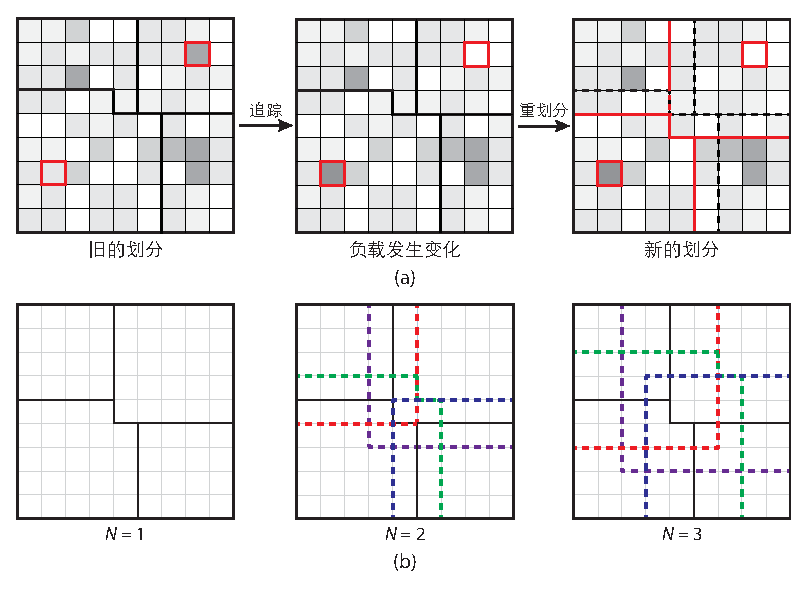
\includegraphics[width=.85\linewidth]{image/loadbalance/repartition.eps}
  \caption{
    动态数据重划分流程示例。\parencite{ZhangGYP18}
  }
  \label{fig:dynamicdr:repartition}
\end{figure}

北京大学可视化和可视分析小组提出了一种基于负载感知的数据重划分的方法\parencite{ZhangGYP18},可以动态地平衡并行粒子追踪过程中的负载,有效地了解决流场计算中的负载平衡问题。
相较于静态负载平衡方法,
这里所提出的方法在初始时使用一般的数据划分和分配策略,不会带来任何预处理开销。
运行时过程被管理为若干个轮次,其目的是平衡每一轮的粒子追踪计算。
在每一轮的追踪之前(除去第一轮),
算法会根据每个数据块的历史负载信息和其中未完成粒子的分布,
动态地评估该轮中每个数据块的负载。
基于负载评估的结果,算法可以执行数据重划分操作,
使得每个进程可以被重新划分和分配到一定的数据块,并继续下一轮的粒子追踪计算。

由于数据冲划分操作会造成一定的开销,
该方法通过适当增大每一轮中的负载,来减小数据重划分的频率。
该方法同时定义在每一轮中每个粒子可以穿过多个数据块,
在负载评估时统计粒子在所有这些数据块上的负载,用于随后的数据划分。
在这样的设定下,可能会出现同一轮中不在同一个起始数据块的粒子会经过相同的数据块的情况,
而这些粒子是可能会被分配给不同的进程的。
因此,为了保证划分后每个进程能够进行独立的粒子追踪,
该方法允许进程之间出现数据重叠。
为了达到这一目的,
该方法在运行时动态地建立了一个图模型,根据粒子的历史数据访问信息记录数据块之间的一阶访问依赖,
用于在负载评估过程中预测从一个数据块到另一个数据块的粒子转移数目,这一操作在每一轮追踪前对未完成粒子被执行。

基于数据重划分管理策略的动态负载平衡方法既可以被用到定常流场中用于计算流线,也可以被用在非定常流场中进行迹线计算。
对于定常流场中的流线计算,
数据只需要被所有进程按照初始划分策略一次性载入,并在数据重划分之后进行交换。
对于非定常流场中的迹线计算,
由于数据包含多个时间步,往往会超出内存的限制,
该方法将其划分为若干个时间步区间,并依次载入处理,使得每个时刻内存中只有一个时间步区间。
每个时间步区间实际上可以被视为具有相同时间维度的定常流场,
因此该方法可以使用和定常流场中的相同方式来处理其粒子追踪和数据重划分操作。

\begin{figure}[H]
%\setlength{\abovecaptionskip}{0.05cm} 
%\setlength{\belowcaptionskip}{-0.20cm}
  \centering
  \includegraphics[width=\linewidth,keepaspectratio]{image/loadbalance/workflow.eps}
  \caption{
    并行粒子追踪计算框架的工作流程。\parencite{ZhangGYP18}
    从对原始数据的初始划分和分配开始,
    该方法通过一个多轮的过程对粒子进行追踪计算。
    在每一轮追踪结束后执行动态数据重划分操作,并按照新的数据分配方案继续下一轮的粒子追踪,
    直至所有粒子完成计算。
 }
\label{fig:dynamicdr:workflow}
\end{figure}

图\ref{fig:dynamicdr:workflow}给出了该方法中的并行粒子追踪计算框架。
给定初始的流场数据划分和粒子种子,
接着就可以开始并行粒子追踪计算。
追踪过程被管理为一个多轮的计算过程。
在每一轮追踪完成后,该方法对所有数据块在下一轮的负载进行动态评估,以此来重划分数据。
之后,算法按照重划分方案将数据和未完成粒子在进程间进行交换,并开始下一轮的粒子追踪计算。

在每一轮中,每个进程独立地进行粒子追踪计算。
为了确保每个进程能有相近的计算时间,每一轮进程的工作负载分布需要尽量均衡,
否则总会有一些进程在等待其他繁忙进程结束本轮计算,造成负载不平衡现象。
因此,如何保持每一轮的负载均衡是非常关键的,也是该方法进行动态数据重划分的目标。 

在每一轮粒子追踪计算完成后,如果还有未完成粒子,
该方法执行数据重划分操作,以期平衡随后的一轮中进程的负载。
具体来说,该方法通过动态地评估每个数据块中未完成粒子在下一轮中的负载,
之后通过对数据进行重划分将其重新分配给进程。
由于非定常流场可看作是多个不同时间步区间下的定常流场,
本文将在定常流场中进行数据重划分作为一般情况来对本章工作进行描述。

该方法同样使用粒子追踪的积分步数来衡量工作负载。
在每一轮中,数据块的负载被定义为所有粒子在该轮中在此数据块内被追踪的步数的总和。
由于每个进程对应一个数据划分,包含了若干数据块,因此其负载也是这些数据块的负载之和。
该方法需要评估每一轮中每个数据块的负载(第一轮除外),
从而可以根据评估结果使用数据重划分方法平衡各个进程的负载。

该工作同时将粒子数目和其历史负载进行考虑,用于预估数据块在每一轮中的负载。
在运行时该方法记录在每个数据块中追踪过的粒子数目和积分步数,并将其作为历史追踪信息附加在这个数据块中。
当一轮粒子追踪结束时,
该方法可以计算每个数据块中粒子的平均负载。
同时,根据未完成粒子的坐标,该方法同时可以获知它们接下来在所有数据块中的分布数量。
因此,每个数据块在下一轮的负载可以用如下方法评估得到。
假设在第$j-1$轮追踪结束之后,算法希望评估第$j$轮的负载。
对于每一个数据块$k$,如果在第$j$轮有$n_{k,j}$个粒子以它为起始块,
那么其预估负载可以使用如下公式进行计算:
\begin{equation}
\label{equ:dynamicdr:estimate}
\begin{aligned}
\overline{w_{k,j}}(n_{k,j})\ =\ \frac{\sum\nolimits_{i=0}^{j-1}w_{k,i}}{\sum\nolimits_{i=0}^{j-1}n_{k,i}} \times n_{k,j},
\end{aligned}
\end{equation}
其中,$w_{k,i}$是数据块$k$在前面的第$i\ (i<j)$轮中的实际负载,
$n_{k,i}$是在前面的第$i\ (i<j)$轮中经过数据块$k$的实际粒子数目。

\begin{figure}[!tb]
%\setlength{\abovecaptionskip}{0.05cm} 
%\setlength{\belowcaptionskip}{-0.20cm}
  \centering
  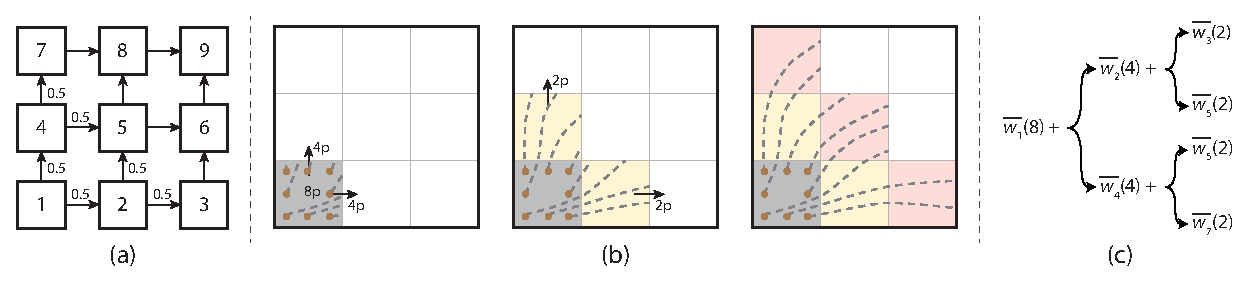
\includegraphics[width=\linewidth]{image/loadbalance/estimate.eps}
  \caption{
    基于ADG的负载评估二维示意图。\parencite{ZhangGYP18}
    (a)在运行时,该方法动态建立访问依赖图;
    (b)对于包含8个粒子的初始数据块1,
    该方法预测在每级追踪深度层次上可能访问的数据块以及粒子在这些数据块中的分布数量,
    这里面数据块之间的箭头表示对粒子下一步走向的预测(箭头边的数字表示粒子转移数量),
    棕色点表示初始粒子,由棕色点出发的虚线表示对粒子追踪情况进行的模拟;
    (c)初始数据块1的预估负载为这8个粒子在(b)中所有数据块中产生的负载的总和。
  }
  \label{fig:dynamicdr:estimate}
\end{figure}

该方法中规定了一个粒子在每轮可以穿过一定数量($N$个)的数据块。
在每一轮中,对于每一个数据块,%从一个数据块开始追踪的粒子,
算法应该评估从该数据块出发的粒子经过$N$个数据块所产生的负载。
当追踪深度$N=1$时,算法只需直接通过公式\ref{equ:dynamicdr:estimate}计算每个数据块的预估负载。
但是当追踪深度$N>1$时,
该方法则还需要知道从一个数据块开始的未完成粒子后面会经过哪些数据块,以及在这些数据块中产生的负载,
才能对这个数据块在这一轮的负载进行全面的评估。
为了达到这个目的,该方法在运行时动态地建立了一个一阶访问依赖图(access dependency graph, ADG)。
在以往的工作中,ADG已经被成功地应用到了有限资源下的流线和迹线计算中\parencite{ChenXLS12,ChenNLS12}。
需要注意的是,这里面该方法没有使用高阶访问依赖的方法,主要是因为高阶访问依赖的计算更为复杂,
而且占用更大的空间,对原本并行粒子追踪的效率影响更大。
在该工作中,每个数据块以多个\texttt{<key, value>}键值对的形式保有ADG的一部分,
其中\texttt{key}是该数据块的邻接块的索引,\texttt{value}是对应的访问转移概率。
在追踪过程中,每个进程计算其所负责的每个数据块关联的访问依赖。
在每一轮粒子追踪结束后,进程通过通信将其计算的ADG的一部分发送到所有其他进程,
使得每个进程都可以获得涵盖所有数据块的完整的ADG。
这种方法可以预测在随后的一轮中
未完成粒子会经过哪些数据块以及粒子在这些数据块中的分布数量。
因此,当追踪深度$N>1$时,根据从初始数据块的访问转移关系,
预测在第二级追踪深度层次上要访问的数据块得以实现。
基于访问转移概率,该方法同样可以预测粒子在这些数据块中的粒子分布数量。
之后,根据公式\ref{equ:dynamicdr:estimate}可以计算得到在每个数据块中的负载。
从这些数据块出发,该方法可以进一步预测在下一级追踪深度层次上要访问的数据块,
直至追踪到第$N$级追踪深度层次。
图\ref{fig:dynamicdr:estimate}展示了追踪深度为3时的负载评估示例。
该方法将初始数据块中的未完成粒子在这些所有涉及到的数据块中的负载累加,
即可得到该初始数据块的预估负载。

在动态负载评估之后,该方法根据对每个数据块的负载评估对数据进行重划分。
在此之前,该方法首先定义一个重划分模型来分析需要解决的问题。
在这个重划分模型中,每个数据块被看作是一个重划分的基本单元和对象,其预估负载被看作是这个对象的权重。

假设原始数据被划分成$m$个数据块,它们分别是$C = \{C_0, C_1, C_2, \cdots, C_{m-1}\}$,
在第$k$次数据重划分之前(即在进行了$k$轮的粒子追踪之后),
对这些数据块的预估负载分别为$w_{k} = \{w_{k,0}, w_{k,1}, w_{k,2}, \cdots, w_{k,m-1}\}$。
对于$n$个进程,算法需要将这些数据块划分为$n$个组,即$G = \{G_0, G_1, G_2, \cdots, G_{n-1}\}$,
其中$G_i = \{C_{i_0}, C_{i_1}, C_{i_2}, \cdots\}$。
每一组的负载是其所包含的所有数据块的负载之和:
$w_{k,{G_i}} = w_{k,{i_0}} + w_{k,{i_1}} + w_{k,{i_2}} + \cdots$。
为了达到负载均衡的目的,划分后的数据块组需要有近似相同的负载。
这里引出了一个最优化问题:最小化每两个数据块组之间的负载差异,即:
\begin{equation}
\label{eqt:dynamicdr:optimization}
\begin{aligned}
  \textrm{min}\ \mathcal{W}_k = \sum_{i=0}^{n-1}\left|w_{k,{G_i}} - \frac{1}{n}\sum_{j=0}^{n-1}w_{k,{G_j}}\right|.
\end{aligned}
\end{equation}

对于数据重划分,这个最优化问题也有一个限制条件。
为了减小重划分之后进程之间的数据交换,
新旧划分之间的重叠必须要尽可能大,也即是新的划分方案
相较于原来的划分方案不应该有显著的变动。

在该工作中,并行粒子追踪框架同时可以用于计算定常流场中的流线和非定常流场中的迹线。
上面描述的方法可以直接应用于定常流场数据。
对于非定常流场,数据块同时包含了空间和时间的维度。
该方法按照先后顺序载入和处理每个时间步区间的数据。
在一个时间步区间中,由于时间维度都是相同的,其数据可以看作是空间块,同时假定相邻时间步的数据具有一定的时间相关性。
对于每一个时间步区间,该方法建立一个新的ADG,并将其用于评估负载和执行数据重划分操作。
这一过程和在定常流场中的做法一致。
当一个时间步区间完成后,该方法根据上一次的重划分结果载入下一个时间步区间,当前的时间步区间则会从内存中清除。
使用这种方法,所有数据不必一次性读取,提高了内存效率。

在执行动态数据重划分时,该方法也使用了一些策略来提高计算的整体性能。
首先,算法适当减小了第一轮的粒子追踪步数。
第一轮只采用了一般的数据划分和分配方法,因此其负载平衡无法保证。
%因此当第一轮的负载比较大时,进程间负载失衡的可能性也在增加。
其次,当未完成粒子的总数比较小时,该方法不执行数据重划分操作。
数据重划分会导致数据在进程间的移动,带来额外的开销。
这种开销有可能会超过由数据重划分带来的性能增益,特别是在最后几轮剩余粒子数非常少的时候。在这种情况下,执行数据重划分操作并不划算。

总的来看,这些方法使用不同的策略,从不同方面一定程度上解决了数据管理方面的问题。
不过,它们在试图提高并行粒子追踪过程中的I/O效率和负载均衡性等影响性能的因素的同时,也带来了各种预处理和运行时过程中其他方面的耗费,
不可避免地会影响并行粒子追踪的整体性能和可扩展性。
从这一方面看,
大规模流场可视化数据管理还需要处理在提高并行粒子追踪性能的同时又会带来其他耗费这两者之间的矛盾。
如何平衡这两个方面的矛盾也是针对大规模流场可视化的数据管理需要考虑的问题。

\subsection{混合并行的流场可视化中的针对负载均衡问题的经典解决方案}
任务并行和数据并行方法在不同的角度上改善了并行粒子追踪的可扩展性,
但是它们在某些方面也都有各自的局限性。%,如表\ref{table:background:comparison}所示。
近年来,研究者们将这两种并行策略结合起来,
提出了混合并行的方法,以期能够进一步提高并行粒子追踪计算的性能。
 
 
\begin{figure}[!tb]
  \centering
  \includegraphics[width=1.0\linewidth]{image/loadbalance/dstep.eps}
  \caption{
    基于DStep框架的混合并行粒子追踪计算\parencite{KendallWAPHE11}。
  }
  \label{fig:background:dstep}
\end{figure}

DStep\parencite{KendallWAPHE11}是由Kendall等人提出的一种类似于
MapReduce\parencite{JeffreyS08}的框架,
可用于解决并行域遍历问题,包括并行粒子追踪的计算(如图\ref{fig:background:dstep}所示)。
DStep有效地结合了两种并行策略的优点:
在数据并行方面,使用轮转的方式静态划分数据;
在任务并行方面,使用基于专有任务队列的任务管理来完成不同类型的任务;
这些都使其进一步提高了并行粒子追踪的可扩展性。
此外,DStep在预处理和运行时都没有特殊的需求,因而非常适用于粒子追踪的并行计算。
研究表明,该框架在超过6万个BlueGene/P核的并行计算环境下仍然具有比较好的性能。
在该工作的基础上,北京大学可视化小组的Guo等人\parencite{GuoYHZ13}和Liu等人\parencite{LiuGZY16}继承了DStep框架并进行了重新设计,
用于在集合模拟数据中生成和管理大规模的迹线,
使系统能够在有限的内存资源环境下运行,同时可以平衡吞吐率和负载均衡之间的关系。
随后,为了将拉格朗日属性空间的投影引入到多变量流场数据的分析上,
Guo等人\parencite{GuoHSZHY14}还进一步改进了DStep框架,
将其与Pivot MDS投影算法\parencite{BrandesP06}集成,
可以支持大规模的并行迹线计算和分析。
这些工作都获得了很好的可扩展性。

混合并行方法充分结合了任务并行和数据并行的优势,能够克服两者固有的一些缺点。
混合并行不需要任何的预处理分析。
由于增加了设计和实现上的复杂性,针对粒子追踪计算的混合并行方法也给研究人员提出了更高的要求。
不过,针对一些特定应用
我们可以充分利用所要解决问题的性质,研究合适的混合并行计算策略。

\subsection{小结}
该小节针对当下大规模科学数据的分析探索中采用的并行计算框架内部中的负载均衡问题做出了深刻的分析和探讨,论述了负载均衡问题对于并行计算的重要性。针对大规模流场可视化中存在的问题,该部分进一步明确了并行粒子追踪任务过程中,具体的负载均衡问题产生的原因和本质,并据此提出了基于动态负载评估和基于K-D树划分的两种改善并行粒子追踪过程中负载不平衡问题的行之有效的解决策略。负载均衡问题是大规模科学数据中采用并行计算手段
中的核心问题,对其诊断和改良因而具有十分重要的意义,是大规模数据管理策略中不可缺少的重要组成部分。


\clearpage
\section{数据约减策略}
随着高性能计算技术的发展,尤其在气象模拟、海洋洋流模拟以及计算流体动力学等研究领域,计算生成的数据规模越来越大,复杂性越来越高。使用现有可视化方法对这些数据进行分析变得更加困难,甚至一些数据集大到无法存储。这对大量数据可视化提出了新的机遇与挑战,包括对数据的存储、管理以及访问。数据约减(压缩)是一种常用的数据管理手段,它通过减少数据的体量来增加研究人员对大规模数据的分析能力。
\subsection{体数据可视化中的数据压缩技术}
为了可视化或分析大规模科学数据,压缩是最有用的技术之一。在科学可视化中,压缩技术主要应用于体数据。 1994年,Tao等人提出了一种基于小波的压缩方法\cite{tao1994progressive},它通过无损压缩保持高精度的数据。Ratanaworabhan等人提出了一种基于快速哈希表查找预测的科学浮点数据的快速无损压缩方法\cite{ratanaworabhan2006fast}。Fout等人通过提出一种基于自适应预测的方法\cite{fout2012adaptive}改进了基于预测的压缩方法。为了提高压缩比,JPEG2000\cite{usevitch2005jpeg2000}是一种通用的方法,提供无损和有损模式。另一种有效且快速的压缩方法是fpzip算法\cite{isenburg2005lossless},它适用于各种整数数据集。最近有人提出了zfp算法\cite{lindstrom2014fixed},它是一种几乎无损的方法,允许用户指定精度,并支持随机块访问。为了加快压缩速度,并行化压缩方法也是一种有效的方法\cite{bi20142}。也有对路径进行压缩的工作\cite{ellsworth2004interactive},在这项工作中使用了基于预测的无损算法,它将粒子的存储量减少了41%,并使粒子检索速度提高了约20%。F. Hong等人提出了一种分层和混合压缩方案\cite{hong2017compression},利用八叉树空间划分来自适应地平衡高压缩比、误差和低减压成本。

\subsection{大规模流场可视化中的数据压缩技术}
在气象模拟、海洋洋流模拟、计算流体力学这些领域中,需要对大规模流场数据进行场线追踪与可视化,数据访问往往是造成性能瓶颈的主要因素之一。越来越大的数据访问需求与I/O带宽和内存等资源的有限性形成了巨大的矛盾。因此,需要更加高效的数据管理与访问方法,在有限资源的条件下,提高场线处理的性能与可扩展性。鉴于对场线追踪时的扩散特性,例如数据访问的稀疏性与局部性,可以对数据访问的模式进行特征抽取,通过对这些抽取的模式进行分析,设计更加高效的稀疏数据管理方法,这些方法不仅需要大大节约场线分析所需的计算资源,还需要提高场线分析的可扩展性。

对于大规模流场数据的可视化,较低的I/O带宽等限制和频繁的数据访问需求之间的不平衡已然成为了场线计算的瓶颈,因此亟需一种对于原始数据的压缩化表达形式以高效生成结果。
最直接的一个方法是将粒子追踪的结果预先保存下来,然后在接下来的应用中随取随用。早在2001年,Bruckschen等人就尝试使用该方式在最小化CPU和内存的使用下
获得实时的粒子追踪的可视化\parencite{BruckschenKHJ01}。这种方法需要预先从规则网格的种子点出发计算出大量的脉线并保存到硬盘中。然后,在交互可视化阶段再根据需要从硬盘中快速地抽取一部分脉线的子集并进行渲染。类似的方法随后也被用到了TB级计算流体动力学数据集的脉线可视化中\parencite{EllsworthGM04}。但是,这种方法并没有考虑特定的应用需求,会带来巨大的预处理开销。研究者更多地将目光转向对流场数据的组织和管理上,通过改变数据原有的存储和表达方式,来达成提升计算效率的目标。

事实上,每条场线都记录了其对应的数据访问信息,即数据的访问依赖关系。因此,算法可以事先计算并记录下这些访问依赖关系,据此指导之后的场线计算,例如对粒子的轨迹进行预测进而预取计算所需的数据。在之前的工作中,研究者们使用了一阶的访问依赖关系来计算流线和迹线,并以此设计了平衡工作负载的方法。但是,这些方法计算的仅仅是从当前访问的数据块到其相邻数据块的访问转移概率,场线的历史数据访问信息并没有加以考虑。如果运用高阶转移的思想,在计算访问依赖关系时结合场线的数据访问历史,就可以得到更精确和可靠的数据访问模式,从而给场线计算应用提供更高效的帮助。

在复杂流场可视化中,基于场线的分析是重要的一类方法,例如迹线流线直接可视化、FTLE计算、源汇查询等。通常在这些分析中,对场线的计算消耗了大量的时间。尽管对于大规模的复杂流场已经有一些高扩展性的算法,但这些方法仍然具有非常高的时间以及I/O代价。然而,对于同一数据的多种可视化与分析方法,其计算所需的场线数据通常是有重合了。这意味着通过粒子追踪得到的场线是有着高度的复用价值的,但在已有的方法中,这些场线则通常被当作“一次性的”。究其原因还是在于场线的规模要比原始流场大出若干个数量级,而导致难以持久存储在硬盘上。如果能对这些场线进行有效管理,并提供高效的访问手段,那么这些场线将可以在资源集约的前提下发挥巨大作用。

系集模拟可视化帮助领域科学家预测和评估模型和参数的不确定性,如追踪全球污染扩散、对比不同发展情形下的气候变化趋势等。然而,受限于数据的复杂程度与规模,以往的系集模拟的差异分析还停留在针对单值场的阶段,对大规模系集流场的差异分析仍悬而未决。这其中难点有二:一是流场中生成的迹线数量庞大,为计算和内存管理带来巨大挑战;二是不同于迹线之间的对比,对多个复杂流场的综合比较和特征提取还没有很明确的解决方案。基于压缩的迹线管理方法可以用来解决该问题。

引入压缩的机制使得在误差可控制的前提下有能力对大量的迹线进行管理,其次引入八叉树,通过不同层次上的压缩来平衡压缩率与访问代价。相比较于传统基于并行粒子追踪的流场可视化与分析,预期能极大的减少I/O代价与时间花费,并能得到接近于无损的计算结果。同时在面对非结构化网格等复杂形式的流场数据时,也有很大的优势。

除了使用数据压缩可以大大提高流场可视化的数据访问效率,还可以对流场数据的访问的规律与模式进行特征抽取,设计特定的数据管理与访问方法,来提高流场数据分析的效率与可扩展性。对流场可视化中数据访问的观察可以发现,尽管整个流场数据往往非常庞大,但在场线计算时真正使用的数据却非常少,这个现象在大规模并行的可视分析方法中同样存在。 其次,尽管流场的数据访问模式往往被假定为是随机的,但实际上存在一系列的算法可以根据流场扩散特性发现其中的规律,在流场的可视分析过程中找到访问模式,提高数据访问的效率。再次,目前的并行流场可视化方法往往需要对数据进行划分,但粒度较粗。理论上算法可以将粗粒度的数据划分转化为细粒度划分,提高并行场线计算算法中任务调度和通信的粒度,提高性能和可扩展性。基于这些观察和考虑,该方法引入了基于并行键值存储和数据预取的稀疏数据管理方法,减小并行场线计算中的数据访问和内存使用需求,在充分满足计算资源限制的前提下提高并行场线计算的性能和可扩展性。该工作设计的方案首先将工作集数据按照小块的粒度进行管理,每个小块仅包含单个或少量数据单元格。在并行系统设计方面,该方法由两部分组成: (1) 并行键值存储进程,负责管理小块的I/O,记录和使用访问模式,以极大程度地隐藏场线计算中的I/O延迟;(2)场线计算进程(简称计算进程),它们相互独立,以任务并行的方式计算场线。

每个场线计算任务被指定且只指定给某一个计算进程,每个计算进程通过队列管理和调度这些任务。计算进程向并行键值存储进程请求和查询数据,并将这些数据保留在本地的LRU缓存中。根据高阶状态转移的思想,该方法提出一种基于高阶访问依赖关系的方法来对流场数据进行管理。通过密集追踪场线的预处理过程,可以计算出数据块之间的高阶访问转移关系,即在某种历史访问背景下,场线从一个数据块进入到相邻块的访问概率。该方法将这种高阶访问依赖关系运用在并行的场线计算中,结合场线的历史访问信息更为精确地预取数据,从而减小I/O开销,相比于一阶的访问依赖,进一步提高了场线计算的效率。更进一步地,该方法可以对流场数据进行重组,将相互依赖关系强的数据组织在一起,以期获得更为可靠和高效的数据局部性。

数据重组也可以有效的帮助实现高效的流场可视化应用计算。顾名思义是将数据按照一定的非常规方式进行重新组织后再在硬盘上进行存储。
针对大规模的网格数据,研究者将其使用图的方式表示,进而将数据重组转化为图排列问题进行解决,以提高缓存效率\parencite{BogomjakovG01,KarniBG02,YoonLPM05,YoonL06}。
而针对大规模非结构化网格数据的粒子追踪,Ueng等人\parencite{UengSM97}将数据按照八叉树的形式进行重新组织存储,在流线的计算过程中,程序会不断地将所需要的数据块载入到内存,并且使用LRU的策略将内存中很久没用到的数据置换出去。为了避免产生大量的内存碎片,内存空间也会被划分为不同大小的块,以适应不同大小的数据块。使用该方法,每个时刻内存中只保有一小部分的数据,使得流线计算可以在内存较小的单机上进行。除了八叉树的形式,z曲线和希尔伯特曲线也被用来在数据重组过程中创建数据索引\parencite{PascucciF01,NiedermeierS96}。Tchiboukdjian等人\parencite{TchiboukdjianDR10}还提出了一个基于理论复杂性分析的布局算法,将非结构化网格表示成重叠图的形式。此外,数据重组还可以结合数据的访问模式,在运行时利用缓存和预取机制动态地提升I/O性能\parencite{AkandeR13}。

在当前的默认情况下,在不同的流可视化应用程序中会大量重复式地重新计算积分曲线,从而导致不必要的资源成本。例如,在FTLE分析中,当一个用户将参数更改为以前的设置,如果历史记录被丢弃,则需要重新计算迹线。在这种情况下,需要加载数据并对种子重新进行粒子跟踪。积分曲线重用技术的主要障碍是它们的体量,它可能比输入的流场数据大几个数量级。庞大的数据规模使得简单的数据重用方式难以生效。北京大学可视化与可视分析小组提出了一种基于压缩的积分曲线数据重用框架\parencite{hong2017compression}来解决上述的问题,以大大降低其检索成本,特别是在资源有限的环境中。在该方法中,单个曲线和一组曲线被压缩并打包在一起,从而大大降低了存储成本。该方法提出了一种分层和混合压缩方案来同时平衡三个目标,包括高压缩比,可控制的误差和较低的解压缩成本。压缩比是该方法的主要关注点,它使积分曲线具有可控性。信息损失直接影响了具体可视化任务的精度,这对于最终用户来说同样尤为重要。同时考虑时间成本和内存成本在内的解压缩成本也是该方法关注的,其可以提供有效地快速检索支持,能够大大降低检索成本。为了在这些因素之间实现合理的平衡,该方法基于八叉树空间划分针对不同大小的种子块的不同压缩策略。具体来说,该方法使用并组合了积分曲线稀疏表示,浮点数据压缩和八叉树空间划分,以自适应地实现上述目标。

该方法可以极大地改善流场可视化任务。在流场可视化应用中,与直接的粒子追踪方法相比,它们可以用更少的时间从内存直接检索积分曲曲线,通常可以为大型数据集提供数十倍的加速。另一方面,该方法可以轻松地扩展到更复杂的数据,例如非结构化网格等。对于非结构化网格,粒子跟踪比常规网格要慢得多,而基于该方法,无论网格复杂度如何,同样可以提供快速的检索结果。

\begin{figure}[htbp]
	\centering
	\includegraphics[width=.7\columnwidth]{image/linecompress/workflow.eps}
	\caption{
	基于压缩的积分曲线重用框架的流程\parencite{hong2017compression}。
	}
	\label{fig:workflow}
\end{figure}

基于压缩的积分曲线重用框架的可视化流程如图所示。该框架主要包括两部分:压缩和解压缩部分。前一部分只对一个数据集运行一次,采用稠密种子进行对整个流场进行数值积分,然后压缩曲线,并将结果保存到存储结构中。为了减少计算时间,该过程可以在大型计算集群中运行以大大降低处理时间。在运行一次之后,解压缩的模块可以为大型流场计算提供有力的支持,对于该部分的处理算法,同样支持并行计算。

积分曲线压缩是该工作中实现数据重用目标的核心技术,其主要障碍来自大体量中间数据。针对这一计算过程,该工作确定了三个优化目标。

{\bf 高压缩比}\quad
粒子追踪通常需要数百或数千个积分步骤才能生成种子的积分曲线,如果算法将种子放置在每个网格点上,则积分曲线的大小将比原始流场大数百倍或数千倍。在该方法提供的压缩方案中,存储非常需要高压缩比。在以下部分中,该工作使用压缩率进行比较。

{\bf 可控的信息丢失}\quad
压缩算法通常以牺牲数据的精确度为代价来实现高压缩率。信息丢失率低,可以确保可视化结果中不会有太多不确定性。对于各种数据集和可视化任务,最终用户对积分曲线的信息损失可能具有不同的容忍度。该工作希望提供某种机制来帮助控制不同情况下的信息丢失。

{\bf 快速检索}\quad
该工作采用基于压缩的重用框架的目的是使用高效的积分曲线提供程序来替换昂贵的粒子跟踪过程。快速检索是加速可视化应用程序的关键因素。大大降低的检索成本也是该工作对重用框架的主要贡献。

\begin{figure}[htbp]
  \centering
  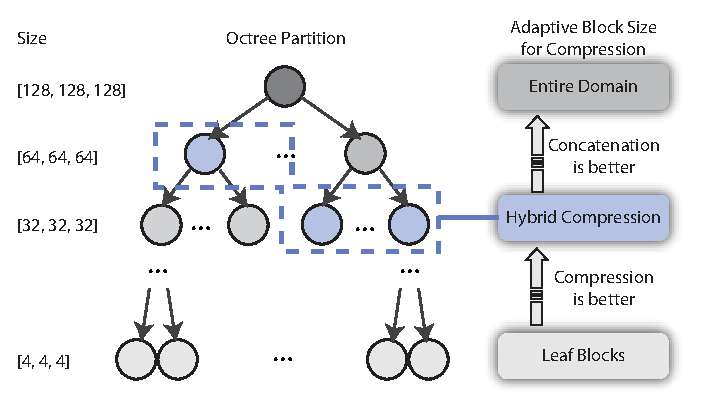
\includegraphics[width=.75\columnwidth]{image/linecompress/recursion.eps}
  \caption{
  基于八叉树空间划分的自适应大小块压缩算法\parencite{hong2017compression}。
  }
  \label{fig:recursion}
\end{figure}

为了平衡上述三个目标,设计了分层和混合压缩方案。具体地,将单独的曲线压缩方法和曲线组压缩方法组合以实现高压缩比并且保持低信息损失。在当前的实现中,该方法分别选择Bezier曲线拟合和fpzip方法。该方法通过将混合压缩方法应用于八叉树划分上的自适应大小的块,以平衡解压缩成本和压缩率。作为一种一般的计算框架,其他压缩算法同样可以代替该实现中的算法,只要在其他压缩算法可以满足上述的目标。

上述的混合压缩仅考虑压缩率与信息丢失之间的权衡。而对于某些方法,例如fpzip库,压缩率和解压缩成本都与块大小高度相关。为了平衡压缩率和解压缩成本,该工作采用八叉树结构将域分层划分为自适应块大小,以进行混合压缩。八叉树空间划分的一种常见用法,其基于某种度量在3D空间中选择合适的细节级别。在该工作框架中,算法自适应地选择更好的块大小以沿八叉树结构进行压缩。具体而言,对于八叉树结构中的一个节点,例如一个种子块,该方法有两种方法来压缩其相应的积分曲线。一种方法是直接应用混合压缩,这有望充分利用所有曲线的空间相干性来获得高压缩率。另一种方法是将其8个子节点(子块)的压缩结果串联为当前块的压缩结果。当仅仅需要稀疏的积分曲线时该方案可以避免解压缩,十分有效。在对每个节点进行选择之后,该工作实际上压缩了多个不同大小的块(蓝色)。对于这些块,该工作将其标识和相应的压缩结果存储在持久存储中以备将来使用。算法的具体流程如图所示。对于上述两种方式的选取,该方法在不同的阈值上进行了多次实验,测量了总压缩比和总解压缩成本。该方式根据经验可以选择了一个阈值,来达成这两种方式优劣的平衡。

\subsection{小结}
该小节综述了大规模科学数据中数据约减的已有核心工作和研究趋势,并以流场可视化中基于压缩的积分曲线重用框架工作为例,详细剖析了数据约减应对可视化或可视分析大规模科学数据流程的挑战的有效性。数据约减策略通过关注大规模数据中的共有趋势或特征,将数据的表示方式加以更变,创造出高效的数据结构和表达形式,以适应可视化和可视分析流程,可以十分有效地减少计算的开销,提升分析和计算结果反馈的实时性,是大规模科学数据管理中重要的组成部分。



\clearpage

\printbibliography[heading = bibintoc]
% \bibliographystyle{plain}
% \bibliography{references.bib}

\end{CJK*}
\end{spacing}
\end{document}
